
% Template for Elsevier CRC journal article
% version 1.2 dated 09 May 2011

% This file (c) 2009-2011 Elsevier Ltd.  Modifications may be freely made,
% provided the edited file is saved under a different name

% This file contains modifications for Procedia Computer Science
% but may easily be adapted to other journals

% Changes since version 1.1
% - added "procedia" option compliant with ecrc.sty version 1.2a
%   (makes the layout approximately the same as the Word CRC template)
% - added example for generating copyright line in abstract

%-----------------------------------------------------------------------------------

%% This template uses the elsarticle.cls document class and the extension package ecrc.sty
%% For full documentation on usage of elsarticle.cls, consult the documentation "elsdoc.pdf"
%% Further resources available at http://www.elsevier.com/latex

%-----------------------------------------------------------------------------------

%%%%%%%%%%%%%%%%%%%%%%%%%%%%%%%%%%%%%%%%%%%%%%%%%%%%%%%%%%%%%%
%%%%%%%%%%%%%%%%%%%%%%%%%%%%%%%%%%%%%%%%%%%%%%%%%%%%%%%%%%%%%%
%%                                                          %%
%% Important note on usage                                  %%
%% -----------------------                                  %%
%% This file should normally be compiled with PDFLaTeX      %%
%% Using standard LaTeX should work but may produce clashes %%
%%                                                          %%
%%%%%%%%%%%%%%%%%%%%%%%%%%%%%%%%%%%%%%%%%%%%%%%%%%%%%%%%%%%%%%
%%%%%%%%%%%%%%%%%%%%%%%%%%%%%%%%%%%%%%%%%%%%%%%%%%%%%%%%%%%%%%

%% The '3p' and 'times' class options of elsarticle are used for Elsevier CRC
%% Add the 'procedia' option to approximate to the Word template
%\documentclass[3p,times,procedia]{elsarticle}
\documentclass[3p,times]{elsarticle}

%% The `ecrc' package must be called to make the CRC functionality available
\usepackage{ecrc}

%% The ecrc package defines commands needed for running heads and logos.
%% For running heads, you can set the journal name, the volume, the starting page and the authors

%% set the volume if you know. Otherwise `00'
\volume{00}

%% set the starting page if not 1
\firstpage{1}

%% Give the name of the journal
\journalname{Robotics and Computer-Integrated Manufacturing}

%% Give the author list to appear in the running head
%% Example \runauth{C.V. Radhakrishnan et al.}
\runauth{Z. Kootbally and  C. Schlenoff and T. Kramer and S.K. Gupta}

%% The choice of journal logo is determined by the \jid and \jnltitlelogo commands.
%% A user-supplied logo with the name <\jid>logo.pdf will be inserted if present.
%% e.g. if \jid{yspmi} the system will look for a file yspmilogo.pdf
%% Otherwise the content of \jnltitlelogo will be set between horizontal lines as a default logo

%% Give the abbreviation of the Journal.  Contact the journal editorial office if in any doubt
\jid{procs}

%% Give a short journal name for the dummy logo (if needed)
\jnltitlelogo{Robotics and Computer-Integrated Manufacturing}

%% Provide the copyright line to appear in the abstract
%% Usage:
%   \CopyrightLine[<text-before-year>]{<year>}{<restt-of-the-copyright-text>}
%   \CopyrightLine[Crown copyright]{2011}{Published by Elsevier Ltd.}
%   \CopyrightLine{2011}{Elsevier Ltd. All rights reserved}
\CopyrightLine{2014}{Published by Elsevier Ltd.}

%% Hereafter the template follows `elsarticle'.
%% For more details see the existing template files elsarticle-template-harv.tex and elsarticle-template-num.tex.

%% Elsevier CRC generally uses a numbered reference style
%% For this, the conventions of elsarticle-template-num.tex should be followed (included below)
%% If using BibTeX, use the style file elsarticle-num.bst

%% End of ecrc-specific commands
%%%%%%%%%%%%%%%%%%%%%%%%%%%%%%%%%%%%%%%%%%%%%%%%%%%%%%%%%%%%%%%%%%%%%%%%%%

%% The amssymb package provides various useful mathematical symbols
\usepackage{amssymb}


%% The amsthm package provides extended theorem environments
%% \usepackage{amsthm}

%% The lineno packages adds line numbers. Start line numbering with
%% \begin{linenumbers}, end it with \end{linenumbers}. Or switch it on
%% for the whole article with \linenumbers after \end{frontmatter}.
%% \usepackage{lineno}

%% natbib.sty is loaded by default. However, natbib options can be
%% provided with \biboptions{...} command. Following options are
%% valid:

%%   round  -  round parentheses are used (default)
%%   square -  square brackets are used   [option]
%%   curly  -  curly braces are used      {option}
%%   angle  -  angle brackets are used    <option>
%%   semicolon  -  multiple citations separated by semi-colon
%%   colon  - same as semicolon, an earlier confusion
%%   comma  -  separated by comma
%%   numbers-  selects numerical citations
%%   super  -  numerical citations as superscripts
%%   sort   -  sorts multiple citations according to order in ref. list
%%   sort&compress   -  like sort, but also compresses numerical citations
%%   compress - compresses without sorting
%%
%% \biboptions{comma,round}

% \biboptions{}

% if you have landscape tables
\usepackage[figuresright]{rotating}

% put your own definitions here:
%   \newcommand{\cZ}{\cal{Z}}
%   \newtheorem{def}{Definition}[section]
%   ...

% add words to TeX's hyphenation exception list
%\hyphenation{author another created financial paper re-commend-ed Post-Script}

% declarations for front matter
\usepackage{verbatim}
\usepackage{moreverb}                    % for boxedboxedverbatim
\usepackage{fancyvrb}
%\usepackage{stfloats}
\usepackage{subcaption}
\usepackage{subfig}

\usepackage[usenames,dvipsnames,svgnames,table]{xcolor}
\usepackage[linesnumbered,boxed,ruled]{algorithm2e}

\newenvironment{mylisting}
{\begin{list}{}{\setlength{\leftmargin}{1em}}\item\small}
{\end{list}}

%%-- mytinylisting
\newenvironment{mytinylisting}
{\begin{list}{}{\setlength{\leftmargin}{1em}}\item\tiny\bfseries}
{\end{list}}

\def\cpp{C{}\texttt{++} }

\begin{document}

\begin{frontmatter}

%% Title, authors and addresses

%% use the tnoteref command within \title for footnotes;
%% use the tnotetext command for the associated footnote;
%% use the fnref command within \author or \address for footnotes;
%% use the fntext command for the associated footnote;
%% use the corref command within \author for corresponding author footnotes;
%% use the cortext command for the associated footnote;
%% use the ead command for the email address,
%% and the form \ead[url] for the home page:
%%
%% \title{Title\tnoteref{label1}}
%% \tnotetext[label1]{}
%% \author{Name\corref{cor1}\fnref{label2}}
%% \ead{email address}
%% \ead[url]{home page}
%% \fntext[label2]{}
%% \cortext[cor1]{}
%% \address{Address\fnref{label3}}
%% \fntext[label3]{}

\dochead{}
%% Use \dochead if there is an article header, e.g. \dochead{Short communication}
%% \dochead can also be used to include a conference title, if directed by the editors
%% e.g. \dochead{17th International Conference on Dynamical Processes in Excited States of Solids}

\title{Towards Robust Assembly with Knowledge Representation for PDDL}

%% use optional labels to link authors explicitly to addresses:
%% \author[label1,label2]{<author name>}
%% \address[label1]{<address>}
%% \address[label2]{<address>}

\author[umd]{Z. Kootbally\corref{cor1}}
\ead{zeid.kootbally@nist.gov}
\author[nist]{C. Schlenoff}
\ead{craig.schlenoff@nist.gov}
\author[cua]{T. Kramer}
\ead{thomas.kramer@nist.gov}
\author[mrc]{S.K. Gupta}
\ead{skgupta@umd.edu}

\address[umd]{University of Maryland, College Park, MD 20740, USA}
\address[nist]{Intelligent Systems Division, National Institute of Standards and Technology, Gaithersburg, MD, USA}
\address[cua]{Department of Mechanical Engineering, Catholic University of America, Washington, DC, USA}
\address[mrc]{Maryland Robotics Center, University of Maryland, College Park, MD, USA}

\cortext[cor1]{Corresponding author: Zeid Kootbally, Department of Mechanical Engineering, University of Maryland, College Park, MD 20740, USA}



\begin{abstract}
The effort described in this paper attempts to integrate agility aspects in the "Agility Performance of Robotic Systems" (APRS) project, developed at the National Institute of Standards and Technology (NIST). The new technical idea for the APRS project is to develop the measurement science in the form of an integrated agility framework enabling manufacturers to assess and assure the agility performance of their robot systems. This framework includes robot agility performance metrics, information models, test methods, and protocols.
This paper presents models for the Planning Domain Definition Language (PDDL), used within the APRS project. PDDL is an attempt to standardize Artificial Intelligence planning languages. The described models have been fully defined in the XML Schema Definition Language (XSDL) and in the Web Ontology Language (OWL) for kit building applications.  Kit building or kitting is a process that brings parts that will be used in assembly operations together in a kit
and then moves the kit to the area where the parts are used in the final assembly. Furthermore, the paper discusses a tool that is capable of automatically and dynamically generating PDDL files from the models in order to replan from scratch or to repair a plan to recover from failures.
\end{abstract}

\begin{keyword}
PDDL (Planning Domain Definition Language) \sep planning \sep replanning \sep plan repair \sep Agility \sep OWL (Web Ontology Language) \sep knowledge representation \sep robotics \sep XSDL (XML Schema Definition Language)
%% keywords here, in the form: keyword \sep keyword

%% PACS codes here, in the form: \PACS code \sep code

%% MSC codes here, in the form: \MSC code \sep code
%% or \MSC[2008] code \sep code (2000 is the default)

\end{keyword}

\end{frontmatter}

%%
%% Start line numbering here if you want
%%
% \linenumbers

%% main text
\section{Introduction}
\label{s:Introduction}
The new technical idea for the ``Agility Performance of Robotic Systems" (APRS) project~\cite{AgilityPerformanceRoboticSystems} at the National Institute of Standards and Technology (NIST) is to develop the measurement science in the form of an integrated agility framework enabling manufacturers to assess and assure the agility performance of their robot systems. This framework includes robot agility performance metrics, information models, test methods, and protocols -- all of which are validated using a combined virtual and real testing environment. The information models enumerate and make explicit the necessary knowledge for achieving rapid re-tasking and being agile and will answer question such as ``What does the robot need to know?", ``When does it need to know it?", and ``How will it get that knowledge?". This framework will (1) allow manufacturers to easily and rapidly reconfigure and re-task robot systems in assembly operations, (2) make robots more accessible to small and medium organizations, (3) provide large organizations greater efficiency in their assembly operations, and (4) allow the U.S. to compete effectively in the global market. Any company that is currently deploying or planning to deploy robot systems will benefit because it will be able to accurately predict the agility performance of its robot systems and be able to quickly re-task and reconfigure its assembly operations.



The increased number of new models and variants have forced manufacturing firms to meet the demands of a diversified customer base by creating products in a short development cycle, yielding low cost, high quality, and sufficient quantity. Modern manufacturing enterprises have two alternatives to face the aforementioned requirements. The first one is to use manufacturing plants with excess capacity and stock of products in inventory to smooth fluctuations in demand. The second one is to use and increase the flexibility of their manufacturing plants to deal with the production volume and variety. While the use of flexibility generates the complexity of its implementation, it still is the preferred solution. Chryssolouris~\cite{Chryssolouris.2005} identified manufacturing flexibility as an important attribute to overcome the increased number of new models and variants from customized demands. Flexibility, however needs to be defined in a quantified fashion before being considered in the decision making process.

Agility is often perceived as combination of speed and flexibility. Gunasekaran~\cite{Gunasekaran.1998} defines agile manufacturing as the capability to survive and prosper in a competitive environment of continuous and unpredictable change by reacting quickly and effectively to changing markets, driven by customer-designed products and services. To be able to respond effectively to changing customer needs in a volatile marketplace means being able to handle variety and introduce new products quickly. Lindbergh~\cite{Lindbergh.1990} and Sharafi \& Zhang~\cite{Sharafi.1999} mentioned that agility consists of flexibility and speed. Essentially, an organisation must be able to \emph{respond flexibly} and \emph{respond speedily}~\cite{Breu.2002}. Conboy \& Fitzgerald~\cite{Conboy.2004} identified terms such as \emph{speed}~\cite{Tan.1998}, \emph{quick}~\cite{DeVor.1995,Kusak.1997,Upton.1994,Yusuf.1999}, \emph{rapid}~\cite{Hong.1996}, and \emph{fast}~\cite{Zain.2003} that occur in most definitions of agility.

The above definitions of agile manufacturing can be applied at the assembly level of a manufacturing system. The assembly system needs to have a certain level of flexibility in the presence of disturbances that can be expressed by the degree of robustness. Kannan \& Parker~\cite{Kannan.2006} described robustness as the ability of the system to identify and recover from faults. Robustness of a control system was described by Leit\~{a}o~\cite{Leitao.2004} as the capability to remain working correctly and relatively stable, even in presence of disturbances. The concept of robustness discussed in this paper is expressed with replanning and plan repair for failure recovery (e.g., misalignments, incorrect parts and tooling, shortage of parts, or missing tool). Fox \textit{et al.}~\cite{Fox.2006} discussed replanning and plan repair when differences are detected between the expected and actual context of execution during plan execution in real environments. The latter authors define plan repair as the work of adapting an existing plan to a new context while perturbing the original plan as little as possible. Replanning is defined as the work of generating a new plan from scratch.

This paper first describes the models developed to represent structures of the planning language in the APRS project. The APRS project is working in collaboration with the IEEE Robotics and Automation Society's Ontologies for Robotics and Automation (ORA) Working Group to develop information models related to kitting, including a model of the kitting environment and a model of a kitting plan. Kitting or kit building is a process that brings parts that will be used in assembly operations together in a kit and then moves the kit to the area where the parts are used in the final assembly. It is anticipated that utilization of the knowledge representation will allow for the development of higher performing kitting systems and will lead to the development of agile automated robot assembly. 

Planning for kitting relies on the Planning Domain Definition Language (PDDL)~\cite{Fox.2003}. In order to operate, the PDDL planners require a PDDL file-set that consists of two files that specify the domain and the problem. From these files, the planning system creates an additional static plan file. Structures of PDDL domain and problem files are fully defined in each of two languages: XML Schema Definition Language (XSDL)~\cite{Walmsley.2002,XMLschemaPrimer,XMLschemaStructures} and Web Ontology Language (OWL) \cite{OWLoverview,OWLspec,OWLprimer}. Furthermore, this paper describes a tool that is capable of automatically and dynamically generating PDDL domain and problem files from the OWL models.




This paper is structured as follows: An overview of the knowledge driven methodology for the APRS project is presented in Section~\ref{section:architecture}. The XSDL models that were developed to represent PDDL domain and problem files are discussed in Section~\ref{section:XML}. A tool that  is capable of automatically and dynamically producing PDDL domain and problem files from OWL files is described in Section~\ref{section:java-tool}. Finally, concluding remarks and future work are addressed in Section~\ref{section:conclusion}.
\section{Knowledge Driven Methodology}
\label{section:architecture}
\begin{figure}[!htb]
\centering
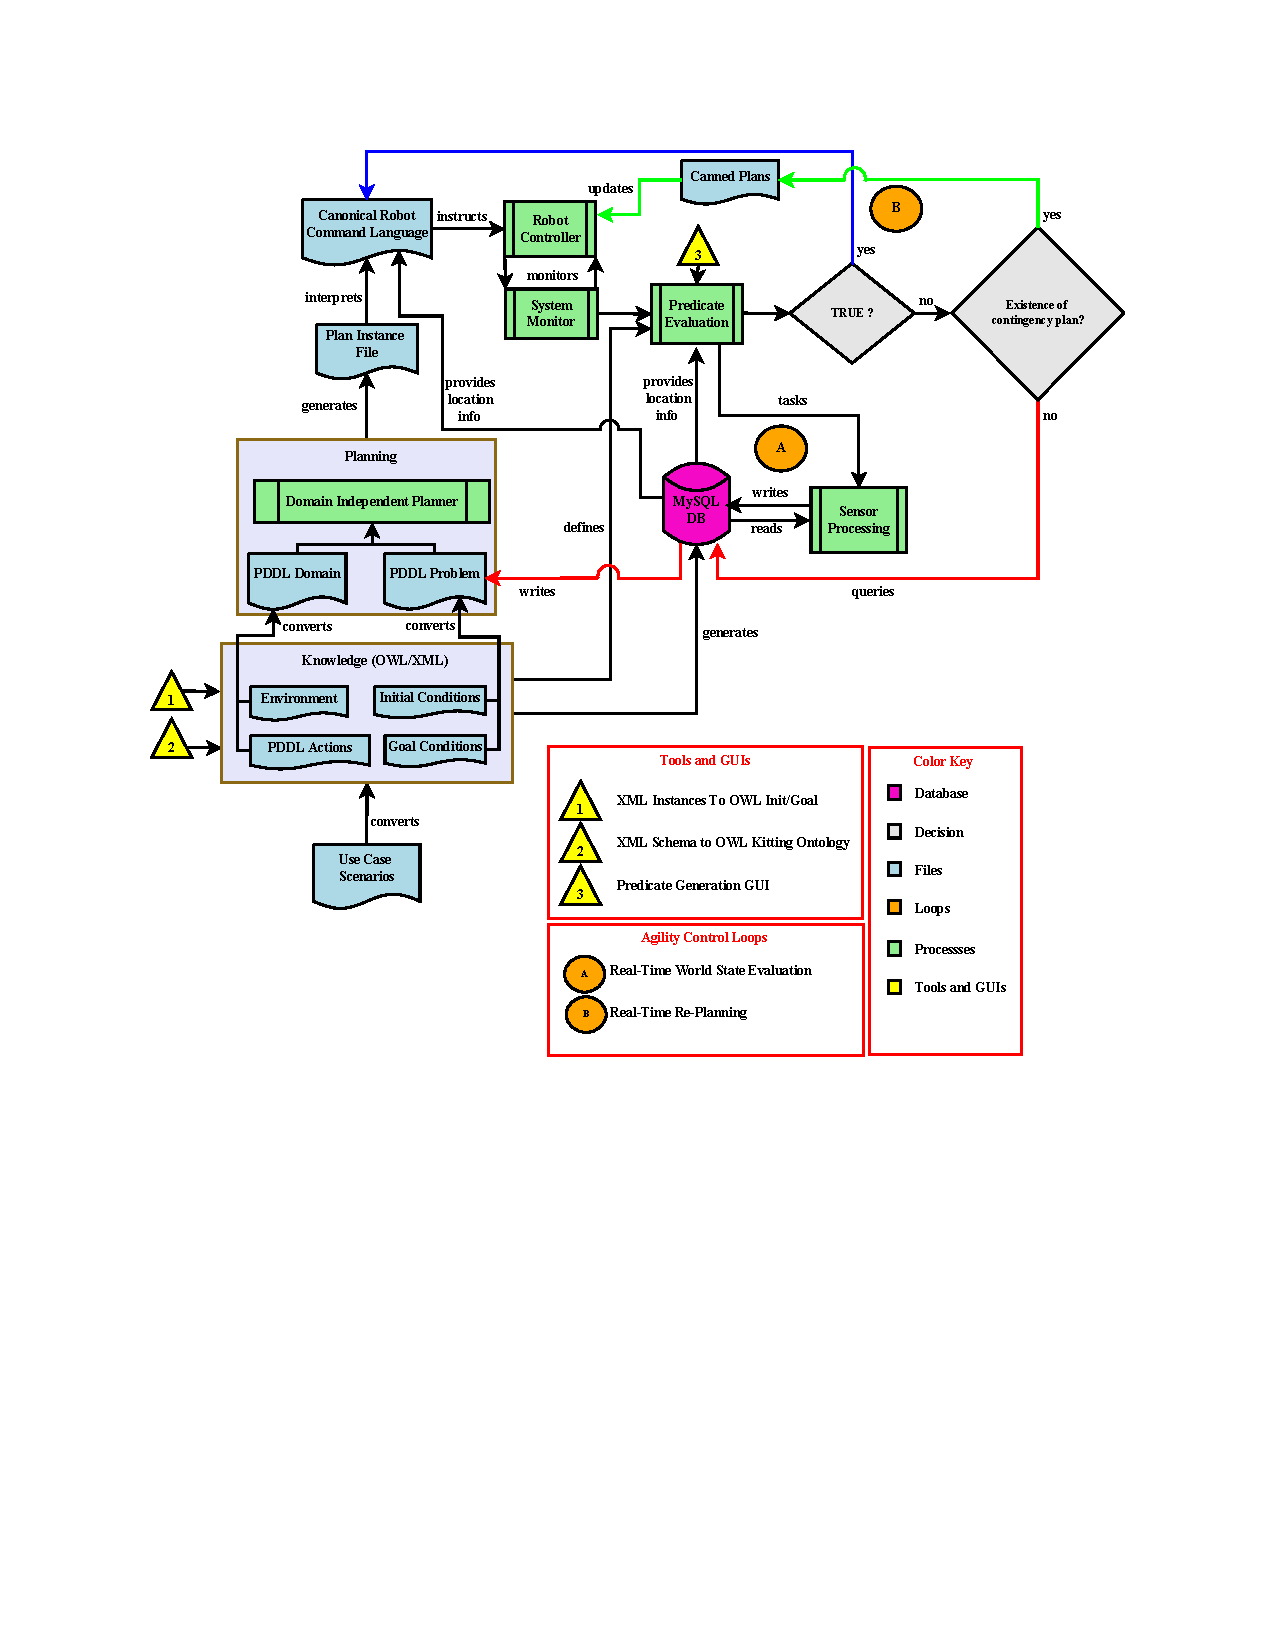
\includegraphics[width=16.5cm]{images/architecture.pdf}
\caption{Knowledge Driven Design extensions.}
\label{fig:methodology}
\end{figure}
The knowledge driven methodology presented in this section is not intended to act as a stand-alone system architecture. Rather it is intended to be an extension to well developed hierarchical, deliberative architectures such as 4D/RCS~\cite{Albus2000}. The overall knowledge driven methodology of the system is depicted in Figure~\ref{fig:methodology}. The remainder of this section gives a brief description of the components pertaining to the effort presented in this paper.
\begin{itemize}
\item \textsf{Use Case Scenarios} -- At the early stage of assembly, new orders coming from customers are entered in the system by an operator via a graphical user interface. The information that is required in this step is for instance the type of assembly and the number of products required. This first step is therefore an attempt to introduce agility in the system with a functionality that smooths fluctuations in demand.

\item \textsf{Knowledge (OWL/XML)} -- At the next level up, the information encoded in the \textsf{Use Case Scenarios} is then organized into a domain independent representation. The \textsf{Knowledge (OWL/XML)} component contains all of the basic information that was determined to be needed during the evaluation of the \textsf{Use Case Scenarios}. This component consists of class files and instance files that describe the environment (\textsf{Environment}), including the initial (\textsf{Initial Conditions}) and goal (\textsf{Goal Conditions}) states for the current assembly, and PDDL actions (\textsf{SOAP}). The knowledge is represented in a compact form with knowledge classes inheriting common attributes from parent classes. The \textsf{SOAP} knowledge describes aspects of PDDL actions that are required for the domain under study. The instance files describe the initial and goal states for the system through the \textsf{Initial Conditions} file and the \textsf{Goal Conditions} file, respectively. The initial state file must contain a description of the environment that is complete enough for a planning system to be able to create a valid sequence of actions that will achieve the given goal state. The goal state file only needs to contain information that is relevant to the end goal of the system.

    Since both the OWL and XML implementations of the knowledge representation are file based, real time information proved to be problematic. In order to solve this problem, an automatically generated MySQL database has been introduced as part of the knowledge representation.

\item \textsf{Planning} -- At the next level up, aspects of this knowledge are automatically extracted and encoded in a form that is optimized for a planning system to utilize. The planning language used in the knowledge driven system is PDDL. The PDDL input format consists of two files that specify the domain and the problem. As shown in Figure~\ref{fig:methodology}, these files are automatically generated from a set of OWL files. The \textsf{PDDL Domain} file is produced from the \textsf{Environment} and the \textsf{SOAP} OWL files while the \textsf{PDDL Problem} file is produced from the \textsf{Initial Condition} and the \textsf{Goal Condition} files. From the \textsf{PDDL Domain} and \textsf{PDDL Problem} files, a domain independent planning system~\cite{Coles.ICAPS.2010} was used to produce a static \textsf{Plan Instance File}.

\item \textsf{Canonical Robot Command Language} -- Once a PDDL plan has been formulated, the knowledge is transformed into a representation that is optimized for use by a robotic system. The interpreter combines knowledge from the PDDL plan with knowledge from the MySQL database to form a sequence of low level commands that the robot controller is able to execute. The authors devised a canonical robot command language (CRCL) in which such lists can be written. The purpose of the CRCL is to provide generic commands that implement the functionality of typical industrial robots without being specific either to the language of the planning system that makes a plan or to the language used by a robot controller that executes a plan.

\item \textsf{Robot Controller} -- CRCL commands are then sent to the \textsf{Robot Controller}. One PDDL action from the \textsf{Plan Instance File} is interpreted into a set of CRCL commands. Each set of CRCL commands is queued and the oldest entries are processed first (FIFO).


\item \textsf{Predicate Evaluation} -- The \textsf{Predicate Evaluation} process is used to check if the preconditions and effects for a PDDL action are satisfied~\cite{Balakirsky2013}. This process intrinsically identifies failures during the execution of an action by the robot. Each precondition and each effect is a predicate expression that must be respectively validated before and after an action is performed. The world model (the MySQL database) is queried for the pose and class of each relevant parameter for a given predicate. The information returned is the latest knowledge that has been recorded by the sensor processing system and is not guaranteed to be up-to-date. This possibly out-of-date information is used as a prediction of the object's current pose and the knowledge is sent as a focus of attention indicator to the sensor processing system. The sensor processing system is instructed to update the world model with current observations and to compute the supporting relationships necessary for predicate evaluation.

    Two distinct results come out of the \textsf{Predicate Evaluation} process.
     \begin{enumerate}
     \item All predicates within the precondition and effect sections for the current action are true. In this case, the next set of CRCL commands are performed (blue arrow).
     \item At least one predicate within the precondition or effect section is false. This case is considered a failure and two situations are checked. The system provides various known failure modes that could exist for the combination of predicates that were found deficient. It provides the consequences of such a failure occurring, remedial information for such failure, and the chance that this kind of failure could occur. In the case a failure mode is provided for the current failure, \textsf{Canned Plans} are used for failure remediation (green arrows). When no failure modes exist for the failed predicate(s), replanning or plan repair is performed (red arrows). Before replanning or plan repair takes place, the MySQL database is queried in order to build the initial state of the environment in the PDDL problem file. This ensures that the initial state of the environment is properly set with current information that will be used to generate a new plan.
     \end{enumerate}
\end{itemize}


\section{Models for PDDL Domain and Problem}
\label{section:XML}
This section describes XSDL models that were developed to represent PDDL structures for domain and problem files. In this project, a two-step process is required to generate PDDL files: (1) XSDL files and XML instance files are used to generate a set of OWL files, (2) the generated OWL files are then used to produce the PDDL files. 

The reader may ask about the necessity of the first step and may find it odd that the PDDL files are not directly encoded in OWL by a human expert. Moreover, the reader may ask about the necessity of using OWL as an intermediate step to generate PDDL files and why not directly going from the XSDL models to PDDL. As mentioned in the introductory section, the APRS project is working in collaboration with the ORA Working Group to develop information models related to kitting. Early in its existence, the ORA Working Group made a commitment to use OWL for its models. As the authors used OWL, difficulties arose as summarized in~\cite{Balakirsky.NISTIR.2013}. The models being built lent themselves to a more structured object model approach of the sort used in languages such as EXPRESS~\cite{express}, \cpp classes~\cite{c++}, and XSDL. It was decided to use XSDL  as the language for initial modeling in the APRS project and to produce OWL models from the XSDL models. Moreover, one author already had experience with XSDL and was building \cpp software tools for manipulating XML schemas and instance files. To make the translation work easier and more reliable, additional \cpp tools were built for that purpose.
%In order to maintain compatibility with the IEEE working group, the ontology has been fully defined in OWL.




\subsection{PDDL Background and Structure}
Since its first release in 1998 as the problem-specific language for the AIPS-98 planning competition~\cite{Ghallab.1998}, PDDL has become a community standard for the representation and exchange of planning domain models. Although the early days of PDDL showed some dissatisfaction in the community, considerable improvements were made to the language, thus enabling the comparison between systems sharing the standard and increasing the availability of shared planning resources. The introduction of PDDL has facilitated the scientific development of planning~\cite{Fox.2003}.

PDDL 2.1 is used for the effort presented in this paper. PDDL 2.1 offers a revised version from the original version of the syntax for expressing numeric-valued fluents. Gerevini \textit{et al.}~\cite{Gerevini.2008} define a numeric fluent as a state variable over the set $\mathbb{R}$ of real numbers such that there exists at least one domain action that can change its initial value specified in the problem initial state. Fox \& Long~\cite{Fox.2003} proposed a definitive syntax for the expression of numeric fluents. The authors provided some minor revisions to the version proposed by McDermott~\cite{Mcdermott.2000}. Another feature introduced in PDDL 2.1 as an optional field within the specification of problems is a plan metric. Plan metrics specify the basis on which a plan will be evaluated for a given problem. Different optimal plans can be produced with different plan metrics for the same initial and goal states. The use of PDDL 2.1 for the effort presented in this paper was motivated by numeric fluents and plan metrics. Even though the plan metrics feature is not currently used in this effort, it is the intention of the authors to do so as the project grows.


\subsubsection{PDDL Domain File}
\label{ss:PDDLdomainFile}
 The development of XSDL models for PDDL requires the analysis of PDDL domain and problem files structures. Figure~\ref{fig:domain} is an excerpt of the PDDL domain file created for kitting. This excerpt is used only for the purpose of this paper. The complete PDDL domain file for kitting consists of 12 \texttt{types}, 34 \texttt{predicates}, 9 \texttt{functions}, and 10 \texttt{actions}. The structure of a PDDL domain file is separated in sections that are described below:

\begin{figure}[t!h!]
\begin{minipage}{.5\paperwidth}
\begin{mylisting}
\begin{Verbatim}[commandchars=\\\{\},fontsize=\scriptsize, numbers=left, numbersep=2pt]
(define (\textcolor{BrickRed}{domain} kitting-domain)
    (\textcolor{BrickRed}{:requirements} :strips :typing :derived-predicates :action-costs :fluents :equality)
    (\textcolor{BrickRed}{:types}
        EndEffector EndEffectorHolder Kit KitTray
        LargeBoxWithEmptyKitTrays LargeBoxWithKits
        Part PartsTray EndEffectorChangingStation
        Robot StockKeepingUnit WorkTable)
    (\textcolor{BrickRed}{:predicates}
        (endEffector-has-no-heldObject ?endeffector - EndEffector)
        (endEffector-is-for-kitTraySKU ?endeffector - EndEffector ?sku - StockKeepingUnit)
        (endEffector-has-physicalLocation-refObject-robot ?endeffector - EndEffector ?robot - Robot)
        (kitTray-has-skuObject-sku ?kittray - KitTray ?sku - StockKeepingUnit)
        (kitTray-has-physicalLocation-refObject-lbwekt ?kittray - KitTray ?lbwekt - LargeBoxWithEmptyKitTrays)
        (robot-has-endEffector ?robot - Robot ?endeffector - EndEffector)		
        (endEffector-has-heldObject-kitTray ?endeffector - EndEffector ?kittray - KitTray) 				
        (kitTray-has-physicalLocation-refObject-endEffector ?kittray - KitTray ?endeffector - EndEffector))
    (\textcolor{BrickRed}{:functions}
        (quantity-of-parts-in-partstray ?partstray - PartsTray)
        (quantity-of-parts-in-kit ?sku - StockKeepingUnit ?kit - Kit)
        (quantity-of-kittrays-in-lbwekt ?lbwekt - LargeBoxWithEmptyKitTrays)
        (quantity-of-kits-in-lbwk ?lbwk - LargeBoxWithKits)
        (current-quantity-of-parts-in-kit ?kit - Kit)
        (final-quantity-of-parts-in-kit ?kit - Kit)
        (capacity-of-parts-in-kit ?partsku - StockKeepingUnit ?kit - Kit)
        (capacity-of-kits-in-lbwk ?lbwk - LargeBoxWithKits)
        (part-found-flag))
    (\textcolor{BrickRed}{:action} take-kitTray
        \textcolor{BrickRed}{:parameters}(
            ?robot - Robot
            ?kittray - KitTray
            ?lbwekt - LargeBoxWithEmptyKitTrays
            ?endeffector - EndEffector
            ?sku - StockKeepingUnit)
        \textcolor{BrickRed}{:precondition}(and
            (> (quantity-of-kittrays-in-lbwekt ?lbwekt) 0)
            (endEffector-has-no-heldObject ?endeffector)
            (endEffector-is-for-kitTraySKU ?endeffector ?sku)
            (endEffector-has-physicalLocation-refObject-robot ?endeffector ?robot)	
            (kitTray-has-skuObject-sku ?kittray ?sku)
            (kitTray-has-physicalLocation-refObject-lbwekt ?kittray ?lbwekt) 			
            (robot-has-endEffector ?robot ?endeffector))				
        \textcolor{BrickRed}{:effect}(and
            (decrease (quantity-of-kittrays-in-lbwekt ?lbwekt) 1)
            (endEffector-has-heldObject-kitTray ?endeffector ?kittray) 				
            (kitTray-has-physicalLocation-refObject-endEffector ?kittray ?endeffector) 	
            (not (endEffector-has-no-heldObject ?endeffector)) 				
            (not (kitTray-has-physicalLocation-refObject-lbwekt ?kittray ?lbwekt))))
)
\end{Verbatim}
\end{mylisting}
\end{minipage}
\caption{Excerpt of the PDDL domain file for kitting.}
\label{fig:domain}
\end{figure}


\begin{itemize}
\item line 1: The keyword \texttt{domain} signals a planner that this file contains information on the domain. \texttt{kitting-domain} is the name given to the domain in the example.
\item line 2: It can be seen in the example that PDDL includes a syntactic representation of the level of expressivity required in particular domain descriptions through the use of \texttt{requirements} flags. This gives the opportunity for a planning system to reject attempts to plan with domains that make use of more advanced features of the language than the planner can handle.

\item lines 3--7:  Object types have to be declared before they are used in \texttt{predicates} and \texttt{functions}. This is done with the declaration \texttt{(:types $\mathtt{name_1}$ $\ldots$ $\mathtt{name_n}$)}.
\item lines 8--16: The \texttt{predicates} part of a domain definition specify only what are the predicate names used in the domain, and their number of arguments (and argument types, if the domain uses \textsf{typing}). The ``meaning'' of a predicate, in the sense of for what combinations of arguments it can be true and its relationship to other predicates, is determined by the effects that actions in the domain can have on the predicate, and by what instances of the predicate are listed as true in the initial state of the problem definition.
\item lines 17--26: \textsf{functions} are used to declare numeric fluents. Numeric assignments (initial value of each function) are set in the initial state of the problem file and change when an action is executed. The declaration of functions is similar to predicates.
\item lines 27--47: The domain is described in terms of action schemata. An action schemata specifies a way that executing an action affects the state of the world. An action schemata includes \texttt{parameters}, \texttt{preconditions}, and \texttt{effects}. An \texttt{action} is identified by a unique name (\texttt{take-kitTray} at line 27). Each \texttt{parameter} of an \texttt{action} is defined by a name and a type (e.g., at line 29, \texttt{robot} is the name of the parameter and \texttt{Robot} is its type). \texttt{Preconditions} and \texttt{effects} may consist of positive predicates (lines 36--41 and lines 44--45). Only preconditions may contain conditions on numeric expressions (line 35). Conditions on numeric expressions are always comparisons between pairs of numeric expressions. They include comparisons between a function and a number (a positive integer) or comparisons between two functions. Only effects may contain function operations (line 43) and negative predicates (lines 46--47). Function operations are used to update the values of primitive numeric expressions.

\end{itemize}

\subsubsection{PDDL Problem File}
A problem is what a planning system tries to solve. A problem specifies an initial situation and a goal to be achieved. Figure~\ref{fig:problem} is a portion of the PDDL problem file created for kitting. This excerpt shows the different components of a generic PDDL problem file. These components are described below.

\begin{figure}[h!t!]
\begin{minipage}{.5\paperwidth}
\begin{mylisting}
\begin{Verbatim}[commandchars=\\\{\},fontsize=\scriptsize, numbers=left, numbersep=2pt]
(define (\textcolor{BrickRed}{problem} kitting-problem)
    (\textcolor{BrickRed}{:domain} kitting-domain)
    (\textcolor{BrickRed}{:objects}
        robot_1 - Robot
        changing_station_1 - EndEffectorChangingStation
        kit_tray_1 - KitTray
        kit_1 - Kit
        empty_kit_tray_supply - LargeBoxWithEmptyKitTrays
        finished_kit_receiver - LargeBoxWithKits
        work_table_1 - WorkTable
        part_a_tray part_b_tray - PartsTray
        part_a_1 part_b_1 - Part
        part_gripper tray_gripper - EndEffector
        part_gripper_holder tray_gripper_holder - EndEffectorHolder
        stock_keeping_unit_part_a stock_keeping_unit_part_b
        stock_keeping_unit_kit_tray - StockKeepingUnit)
    (\textcolor{BrickRed}{:init}
        (endEffector-has-no-heldObject  part_gripper)
        (endEffector-has-no-heldObject  tray_gripper)
        (endEffector-is-for-kitTraySKU tray_gripper stock_keeping_unit_kit_tray)
        (endEffector-is-for-partSKU part_gripper stock_keeping_unit_part_a)
        (endEffector-is-for-partSKU part_gripper stock_keeping_unit_part_b)
        (endEffectorHolder-has-physicalLocation-refObject-changingStation part_gripper_holder changing_station_1)
        (endEffectorHolder-has-physicalLocation-refObject-changingStation tray_gripper_holder changing_station_1)
        (kitTray-has-skuObject-sku kit_tray_1 stock_keeping_unit_kit_tray)
        (partsVessel-has-part part_a_tray part_a_1)
        (partsVessel-has-part part_b_tray part_b_1)

        (= (quantity-of-parts-in-partstray part_a_tray) 1)
        (= (quantity-of-parts-in-partstray part_b_tray) 1)
        (= (quantity-of-parts-in-kit stock_keeping_unit_part_a kit_1) 0)
        (= (quantity-of-parts-in-kit stock_keeping_unit_part_b kit_1) 0)
        (= (quantity-of-kittrays-in-lbwekt empty_kit_tray_supply) 1)
        (= (quantity-of-kits-in-lbwk finished_kit_receiver) 0)
        (= (capacity-of-parts-in-kit stock_keeping_unit_part_a kit_1) 1)
        (= (capacity-of-parts-in-kit stock_keeping_unit_part_b kit_1) 1)
        (= (capacity-of-kits-in-lbwk finished_kit_receiver) 12)
        (= (current-quantity-of-parts-in-kit kit_1) 0)
        (= (final-quantity-of-parts-in-kit kit_1) 2)
        (= (part-found-flag) 1))
    (\textcolor{BrickRed}{:goal}(and
        (kit-has-physicalLocation-refObject-lbwk kit_1 finished_kit_receiver)
        (lbwk-has-kit finished_kit_receiver kit_1)))
)
\end{Verbatim}
\end{mylisting}
\end{minipage}
\caption{The PDDL problem file for kitting.}
\label{fig:problem}
\end{figure}


\begin{itemize}
\item line 1: The keyword \texttt{problem} signals a planner that this file contains information on the problem. \texttt{kitting-problem} is the name given to the problem in the example.
\item line 2: A problem is defined with respect to a domain. The keyword \texttt{domain} is a reference to the domain to which the problem is associated. In the example, the problem is defined with respect to the domain described in Figure~\ref{fig:domain}.
\item lines 3--16:  \texttt{objects} specifies the distinct instances and types of objects that will appear in the initial and goal states.
\item lines 17--40: The \texttt{init} section consists of predicates that are true in the initial state. Because of the closed world assumption of PDDL, predicates not specified in the \texttt{init} section are set to false. The initial value of each \texttt{function} described in the domain is set in the \texttt{init} section. For instance, line 29 tells the planning system that \textsf{part\_a\_tray} contains 1 part in the initial state. In Figure~\ref{fig:problem}, function assignments are depicted at lines 29--40.
\item lines 41--43: The \texttt{goal} section specifies the predicates that need to be true in the goal state. The value that a \texttt{function} needs to reach may also be specified in the \texttt{goal} section.
\end{itemize}

\subsection{Models for PDDL Domain}
A closer look at Figure~\ref{fig:problem} shows that all the basic components (\texttt{objects}, \texttt{predicates}, and \texttt{functions}) in the problem are also defined in the domain. The only difference is that the problem requires instance parameters while the domain uses generic parameters. Therefore, only the PDDL domain needs to be modeled and the information that goes in the definition of the problem can be mapped in the program.

The authors have modeled the structure of a PDDL domain in the \textsf{SOAP} schema. \textsf{SOAP} stands for States, Ordering constructs, Actions, and Predicates. To remove any confusion on this acronym, the authors need to clarify that models of states, ordering constructs, actions, and predicates were used in a sister project, however, only actions and predicates from the \textsf{SOAP} schema are used in the APRS project.


The \texttt{types} section in the domain and the \texttt{objects} section in the problem contain information that is stored in the \textsf{KittingWorkstation} model. This model is imported by the \textsf{SOAP} model. \textsf{SolidObject} and \textsf{DataThing} constitute the two top-level classes of the \textsf{KittingWorkstation} ontology model, from which all other classes are derived. \textsf{SolidObject} models solid objects, things made of matter. The \textsf{KittingWorkstation} ontology includes several subclasses of \textsf{SolidObject} that are formed from components that are \textsf{SolidObject}. The \textsf{DataThing} class models data for \textsf{SolidObject}. The \textsf{KittingWorkstation} model is fully documented in~\cite{Balakirsky.NISTIR.2013}.



To describe models of PDDL domains in \textsf{SOAP}, the authors will often refer to Figure~\ref{fig:domain}. The different figures of classes presented in the remainder of this section were generated by XMLSpy~\cite{XMLSpyManual}. In these figures, a dotted line around a box means the attribute is optional (may occur zero times), a $0..\infty$ underneath a box means it may not occur, with no upper limit on the number of occurrences, and a $1..\infty$ underneath a box means it may occur at least once, with no upper limit on the number of occurrences. Moreover, the following conventions are adopted in the model descriptions:
\begin{itemize}
\item Elements with the suffix \textsf{Type}: An element in the model with the suffix \textsf{Type} is either a XML schema \textsf{simpleType} or a \textsf{complexType}. The \textsf{simpleType} element defines a simple type and specifies the constraints and information about the values of attributes or text-only elements. The \textsf{complexType} element defines a complex type. A complex type element is an XML element that contains other elements and/or attributes. \textsf{simpleType} and \textsf{complexType} elements are translated into OWL classes.
\item Elements with the suffix \emph{Name}: An element in the model with the suffix \emph{Name} designates that the element refers to either a \textsf{simpleType} or a \textsf{complexType}. Referencing a \textsf{simpleType}/\textsf{complexType} requires that the \textsf{simpleType}/\textsf{complexType} is already defined.
\end{itemize}


\begin{figure}[htb!]
\centering
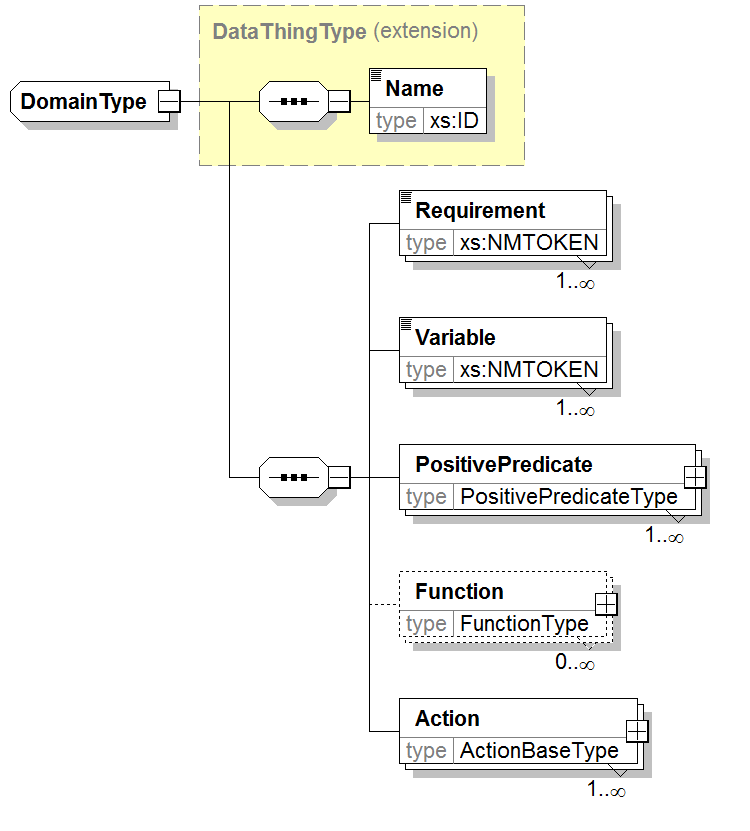
\includegraphics[width=.5\linewidth]{images/XMLSPYDiagrams/DomainType.png}
\caption{\textsf{DomainType} for modeling PDDL domain files.}
\label{fig:DomainType}
\end{figure}

\emph{Domain}: A PDDL domain is modeled with \textsf{DomainType}. \textsf{DomainType} extends \textsf{DataThingType} and consists of a name (inherited), a set of requirements, a set of variables, a set of predicates, an optional set of functions, and a set of actions. These components model a PDDL domain file such as the one shown in Figure~\ref{fig:domain}. Components of  \textsf{DomainType} are described below.
\begin{itemize}
\item \emph{Requirement} and \emph{Variable}: \emph{Requirement} and \emph{Variable} respectively represent the \texttt{requirements} and the \texttt{types} sections in the PDDL domain file. Since the term \textsf{Type} is already used to designate a XSDL type, the PDDL term \texttt{types} was replaced by \emph{Variable}. A \emph{Requirement} and a \emph{Variable} are of type \textsf{xs:NMTOKEN} in XSDL and of type \textsf{string} in OWL.

\item \emph{PositivePredicate}: PDDL predicates are used in positive and negative forms. A PDDL positive predicate is modeled with \textsf{PositivePredicateType}, which is depicted in Figure~\ref{fig:PositivePredicateType}. \textsf{PositivePredicateType} extends \textsf{DataThingType} and consists of a name (inherited), an optional description, a reference parameter, and an optional target parameter. The predicates used in the kitting PDDL domain and problem files all have at least one parameter and can have up to two parameters. In the case a predicate has two parameters, the first parameter is identified as the \emph{ReferenceParameter} and the second parameter is identified as the \emph{TargetParameter}. In the case a predicate has only one parameter, this parameter is identified as the \emph{ReferenceParameter}.

\begin{figure}[h!tb!]
\centering
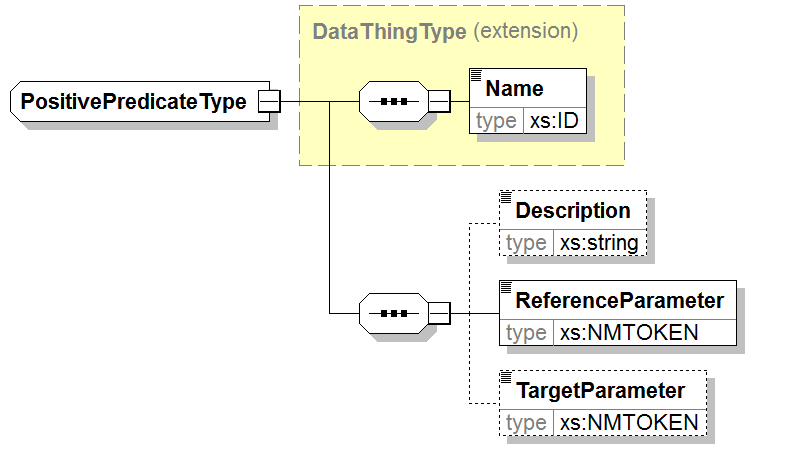
\includegraphics[width=.5\linewidth]{images/XMLSPYDiagrams/PositivePredicateType.png}
\caption{\textsf{PositivePredicateType} for modeling PDDL positive predicates.}
\label{fig:PositivePredicateType}
\end{figure}


\item \emph{Function}: PDDL functions are modeled with \textsf{FunctionType}, which is depicted in Figure~\ref{fig:FunctionType}. \textsf{FunctionType} extends \textsf{DataThingType} and consists of a name (inherited), an optional description, an optional reference parameter, and an optional target parameter. As one can note, the reference and target parameters are both optional for a \textsf{FunctionType} since some PDDL functions in our kitting domain are void of parameters such as \texttt{(part-found-flag)} at line 26 in Figure~\ref{fig:domain}.

    \begin{figure}[h!tb!]
    \centering
    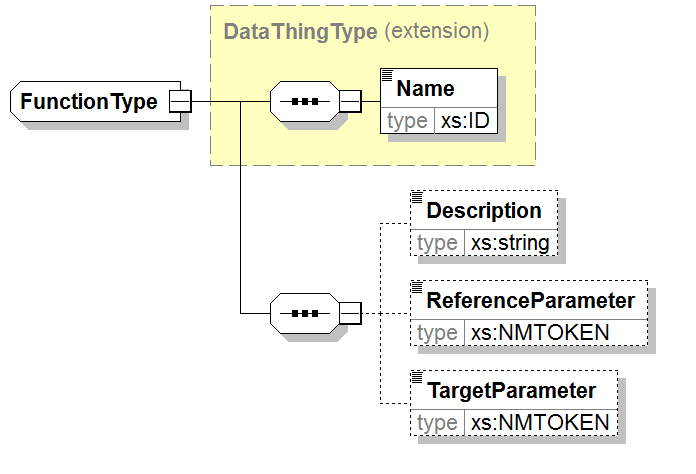
\includegraphics[width=.5\linewidth]{images/XMLSPYDiagrams/FunctionType.png}
\caption{\textsf{FunctionType} for modeling PDDL functions.}
    \label{fig:FunctionType}
    \end{figure}

\item \emph{Action}: PDDL actions are modeled with \textsf{ActionBaseType}, which is depicted in Figure~\ref{fig:ActionBaseType}. \textsf{ActionBaseType} extends \textsf{DataThingType}. \textsf{ActionBaseType} consists of a unique name (inherited), an optional description, a set of parameters, a precondition section, and an effect section. The components of \textsf{ActionBaseType} are described as follows:

    \begin{figure}[htb!]
\centering
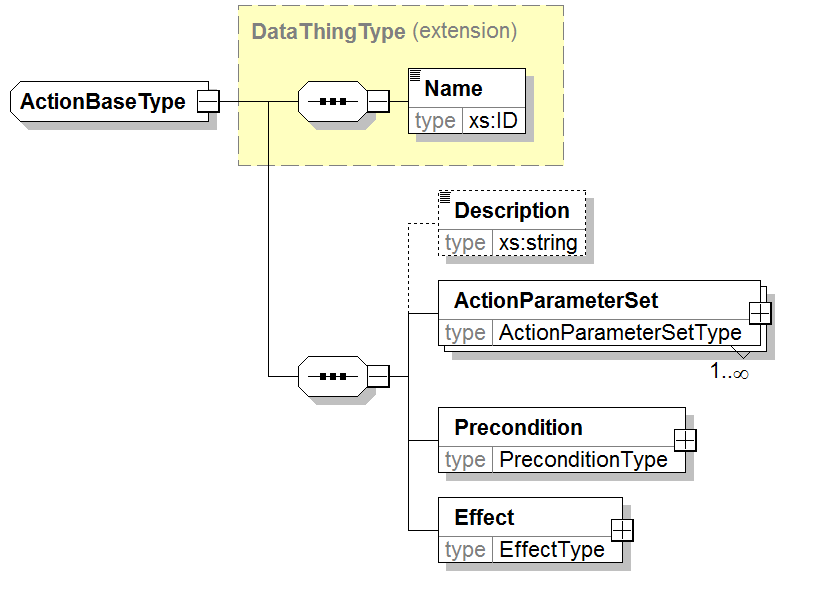
\includegraphics[width=.5\linewidth]{images/XMLSPYDiagrams/ActionBaseType-Collapsed.png}
\caption{\textsf{ActionBaseType} for modeling PDDL actions.}
\label{fig:ActionBaseType}
\end{figure}


\begin{itemize}
\item \emph{Name}: The unique name of a PDDL action is assigned with the inherited name attribute.
\item \emph{Description}: A description is written in the generated PDDL file as a PDDL comment. The purpose of a description is only to inform the user about the role of a PDDL action.
\item \emph{ActionParameterSet}:
    \begin{figure}[htb!]
    \centering
    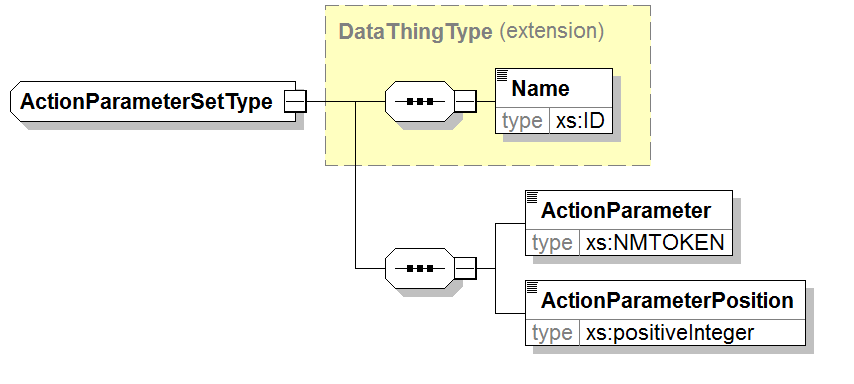
\includegraphics[width=.5\linewidth]{images/XMLSPYDiagrams/ActionParameterSetType.png}
    \caption{\textsf{ActionParameterSetType} for modeling PDDL actions' parameters.}
    \label{fig:ActionParameterSetType}
    \end{figure}
PDDL actions' parameters are modeled with \textsf{ActionParameterSetType} (see Figure~\ref{fig:ActionParameterSetType}). \textsf{ActionParameterSetType} consists of a unique name (inherited), the type of the parameter, which is identified with \emph{ActionParameter}, and the position of the parameter, identified with \emph{ActionParameterPosition}, in the list of parameters for a PDDL action \footnote{The authors are currently using numbers (integers) to represent orders of parameters in a list of parameters as no built-in structure exists for the representation of ordered lists in OWL.}. To illustrate these components, the reader may refer to the action \texttt{take-kitTray} at line 29 in Figure~\ref{fig:domain}.  The action \texttt{take-kitTray} consists of five parameters where each parameter is an \textsf{ActionParameterSetType}. The \emph{ActionParameter} for the parameter \texttt{robot} is \texttt{Robot} and its  \emph{ActionParameterPosition}  is 1.

    \begin{figure}[htb!]
    \centering
    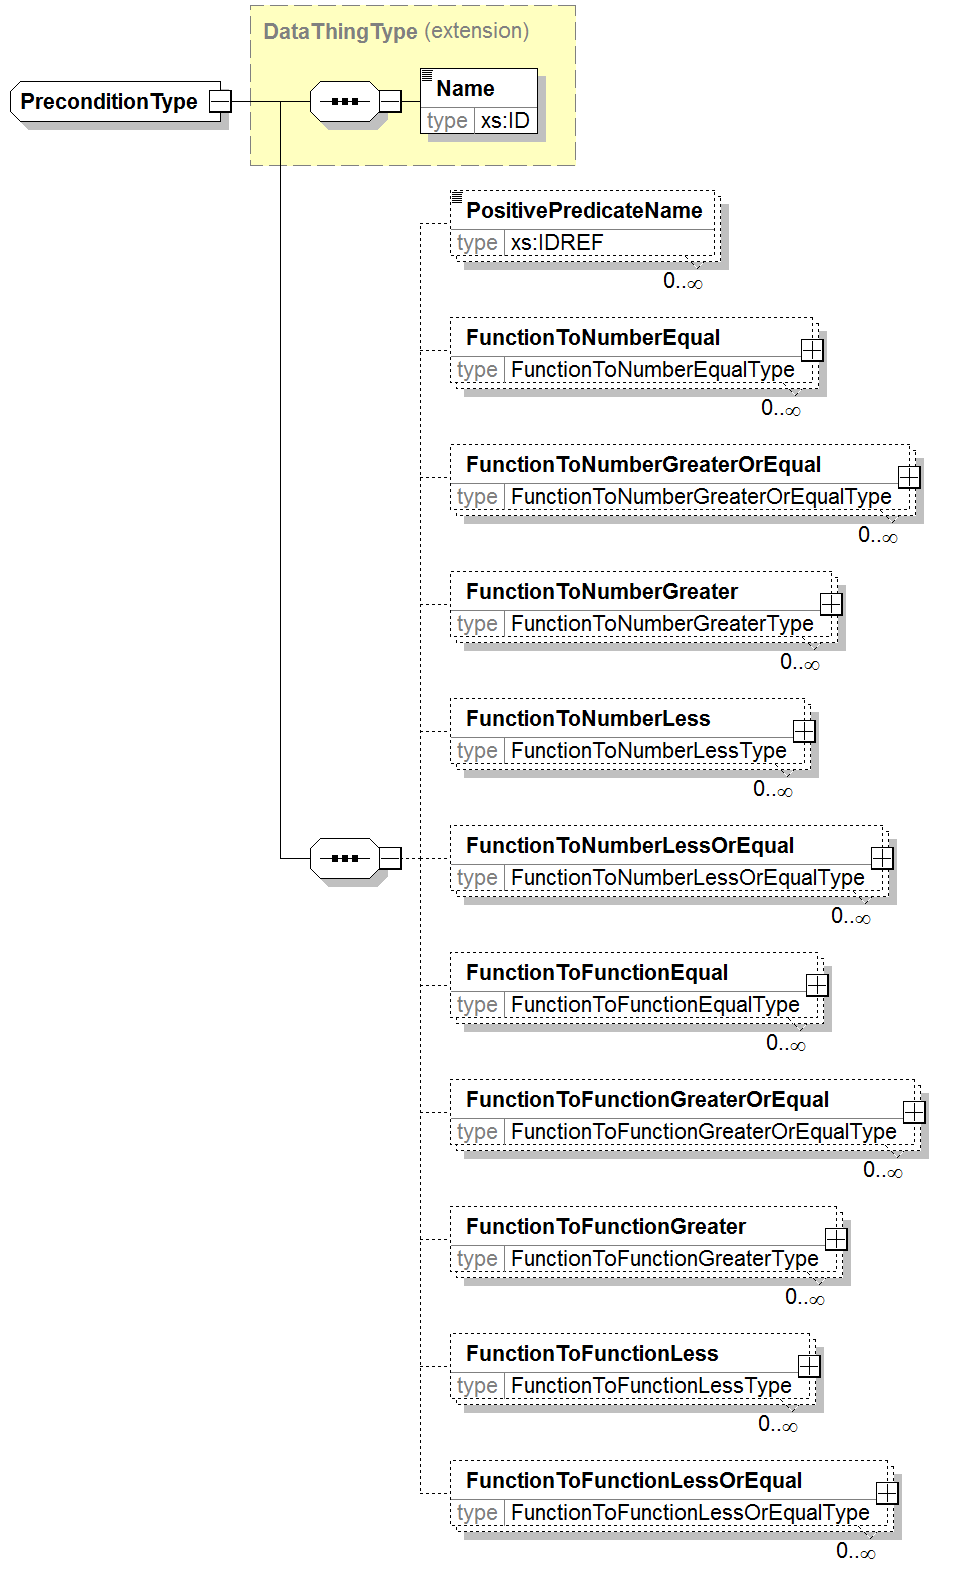
\includegraphics[width=.5\linewidth]{images/XMLSPYDiagrams/PreconditionType.png}
    \caption{\textsf{PreconditionType} for modeling PDDL actions' preconditions.}
    \label{fig:PreconditionType}
    \end{figure}
\item \emph{Precondition}: The precondition section of a PDDL action is modeled with \textsf{PreconditionType}, which is depicted in Figure~\ref{fig:PreconditionType}. A \textsf{PreconditionType} extends \textsf{DataThingType}. A \textsf{PreconditionType} consists of a unique name (inherited), optional references to positive predicates, and optional references to conditions on functions. Components of \textsf{PreconditionType} are summarized below.
\begin{itemize}
\item \emph{Name}: The unique name of a PDDL action's precondition is assigned with the inherited name attribute.
\item \emph{PositivePredicateName}: A \textsf{PositivePredicateName} refers to a \textsf{PositivePredicateType}, meaning that specific \textsf{PositivePredicateType}s need to be declared before they are referenced.
\item Conditions on functions: Conditions on functions are modeled with \textsf{FunctionConditionType}. A \textsf{FunctionConditionType} extends \textsf{DataThingType} and is used to compare two \textsf{FunctionType}s with each other or to compare a \textsf{FunctionType} with a number. Comparisons between two \textsf{FunctionType}s are modeled with \textsf{FunctionToFunctionConditionType}. Comparisons between  a \textsf{FunctionType} and a number are modeled with \textsf{FunctionToNumberConditionType}. More information on \textsf{FunctionToFunctionConditionType} and on \textsf{FunctionToNumberConditionType} is given below.

\begin{itemize}
        \begin{figure}[h!tb!]
        \centering
        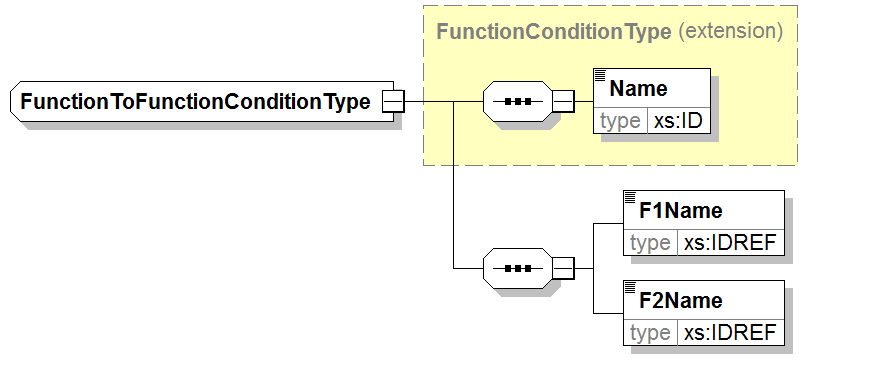
\includegraphics[width=.5\linewidth]{images/XMLSPYDiagrams/FunctionToFunctionConditionType.png}
        \caption{\textsf{FunctionToFunctionConditionType} for comparing two PDDL functions.}
        \label{fig:FunctionToFunctionConditionType}
        \end{figure}
        
                \begin{figure}[h!t!b!]
        \centering
        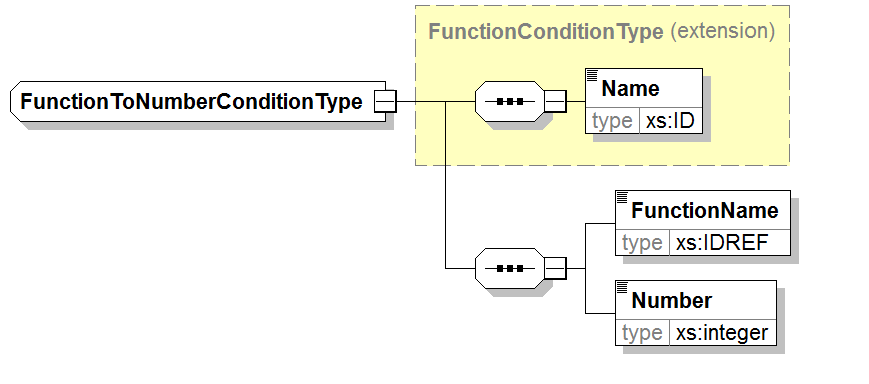
\includegraphics[width=.5\linewidth]{images/XMLSPYDiagrams/FunctionToNumberConditionType.png}
        \caption{\textsf{FunctionToNumberConditionType} for comparing PDDL functions with numbers.}
        \label{fig:FunctionToNumberConditionType}
        \end{figure}
    \item A \textsf{FunctionToFunctionConditionType} extends \textsf{FunctionConditionType} (see Figure~\ref{fig:FunctionToFunctionConditionType}) and consists of a name (inherited), a reference to the first \textsf{FunctionType} (identified with \emph{F1Name}), and a reference to the second \textsf{FunctionType} (identified with \emph{F2Name}). Comparisons between \textsf{FunctionType}s require definitions of mathematical symbols (``$<$", ``$\leq$", ``$=$", ``$\geq$", and `$>$"), which are expressed with subtypes of \textsf{FunctionToFunctionConditionType}. The mapping between mathematical symbols and subtypes of \textsf{FunctionToFunctionConditionType} is performed as follows: ``$<$" is modeled with \textsf{FunctionToFunctionLessType}, ``$\leq$" is modeled with \textsf{FunctionToFunctionLessOrEqualType}, ``$=$" is modeled with \textsf{FunctionToFunctionEqualType}, ``$\geq$" is modeled with \textsf{FunctionToFunctionGreaterOrEqualType}, and ``$>$" is modeled with \textsf{FunctionToFunctionGreaterType}.

    \item A \textsf{FunctionToNumberConditionType} extends \textsf{FunctionConditionType} (see Figure~\ref{fig:FunctionToNumberConditionType}) and consists of a name (inherited), a reference to a \textsf{FunctionType} (identified with \emph{FunctionName}), and a number (identified with \emph{Number}). Similar to \textsf{FunctionToFunctionConditionType}, subtypes of \textsf{FunctionToNumberConditionType} indicates the mathematical symbols used for the comparison between a \textsf{FunctionType} and a number. The mapping between mathematical symbols and subtypes of \textsf{FunctionToNumberConditionType} is performed as follows: ``$<$" is modeled with \textsf{FunctionToNumberLessType}, ``$\leq$" is modeled with \textsf{FunctionToNumberLessOrEqualType}, ``$=$" is modeled with \textsf{FunctionToNumberEqualType}), ``$\geq$" is modeled with \textsf{FunctionToNumberGreaterOrEqualType}, and ``$>$" is modeled with \textsf{FunctionToNumberGreaterType}. An illustration of a \textsf{FunctionToNumberGreaterType} is given at line 35 in Figure~\ref{fig:domain}.
\end{itemize}
%\begin{figure}[htb!]
%        \centering
%        \begin{subfigure}{.5\textwidth}
%        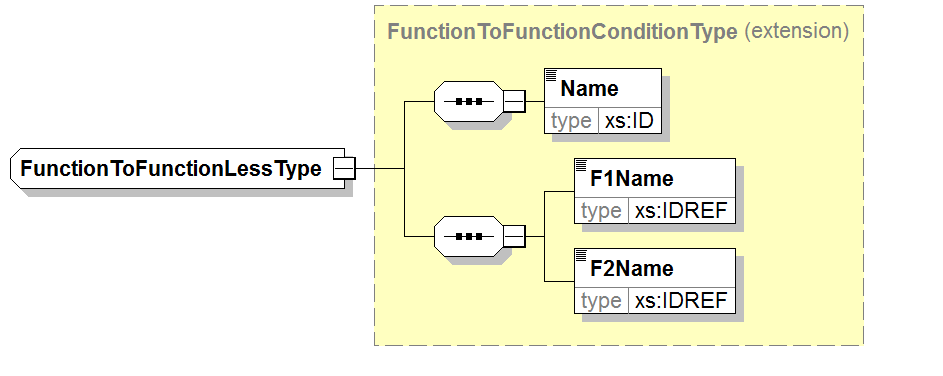
\includegraphics[width=1\linewidth]{images/XMLSPYDiagrams/FunctionToFunctionLessType.png}
%        \caption{\textsf{FunctionToFunctionLessType} for comparing two PDDL functions with each other using the mathematical symbol ``$<$".}
%        \label{fig:FunctionToFunctionLessType}
%        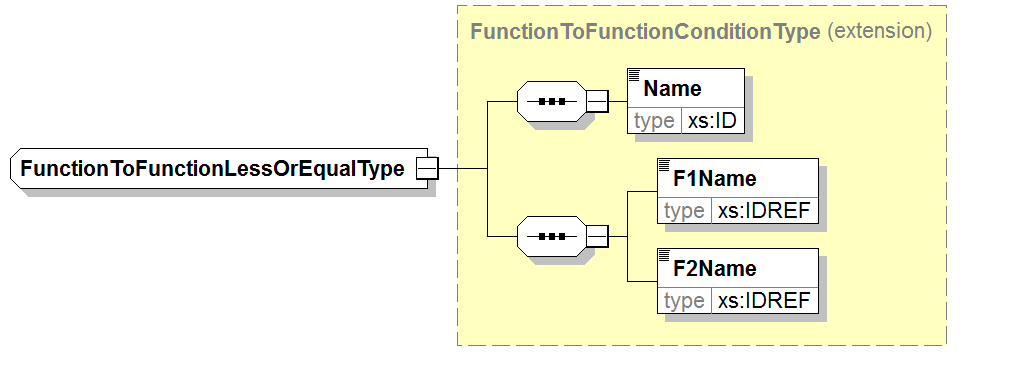
\includegraphics[width=1\linewidth]{images/XMLSPYDiagrams/FunctionToFunctionLessOrEqualType.png}
%        \caption{\textsf{FunctionToFunctionLessOrEqualType} for comparing two PDDL functions with each other using the mathematical symbol ``$\leq$".}
%        \label{fig:FunctionToFunctionLessOrEqualType}
%        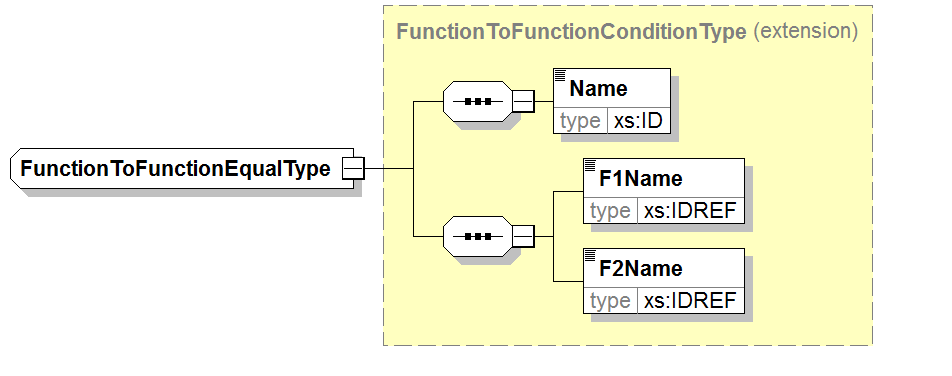
\includegraphics[width=1\linewidth]{images/XMLSPYDiagrams/FunctionToFunctionEqualType.png}
%        \caption{\textsf{FunctionToFunctionEqualType} for comparing two PDDL functions with each other using the mathematical symbol ``$=$".}
%        \label{fig:FunctionToFunctionEqualType}
%        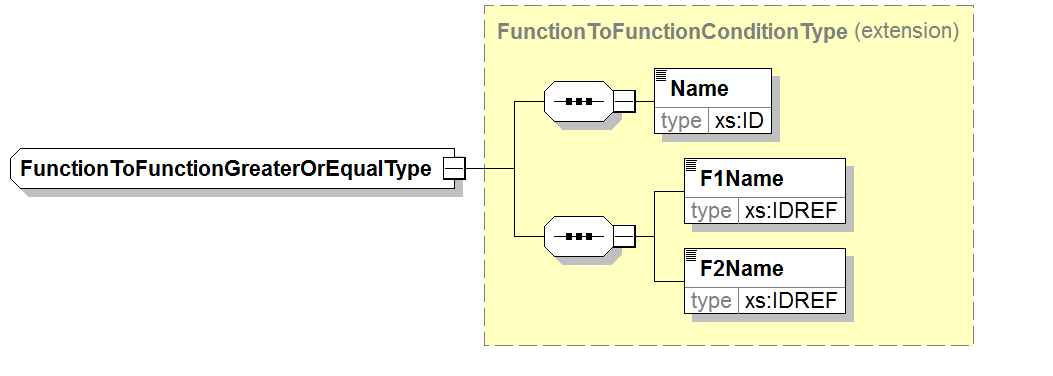
\includegraphics[width=1\linewidth]{images/XMLSPYDiagrams/FunctionToFunctionGreaterOrEqualType.png}
%        \caption{\textsf{FunctionToFunctionGreaterOrEqualType} for comparing two PDDL functions with each other using the mathematical symbol ``$\geq$".}
%        \label{fig:FunctionToFunctionGreaterOrEqualType}
%        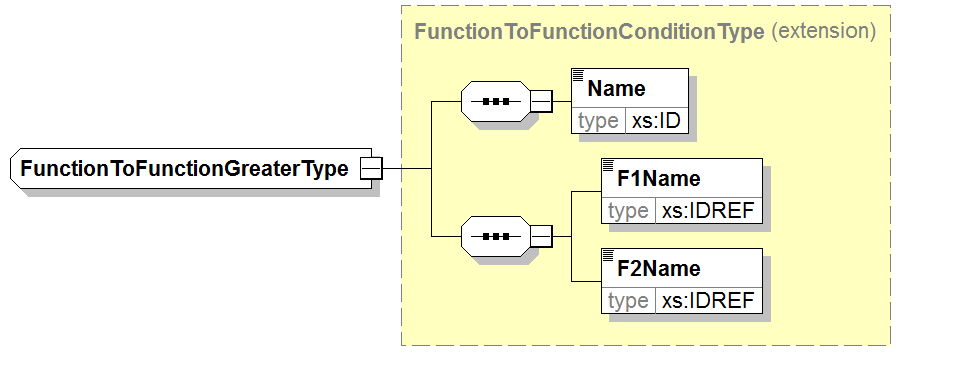
\includegraphics[width=1\linewidth]{images/XMLSPYDiagrams/FunctionToFunctionGreaterType.png}
%        \caption{\textsf{FunctionToFunctionGreaterType} for comparing two PDDL functions with each other using the mathematical symbol ``$>$".}
%        \label{fig:FunctionToFunctionGreaterType}
%        \end{subfigure}
%        \caption{Subtypes of \textsf{FunctionToFunctionConditionType}.}
%        \label{fig:fig}
%        \end{figure}
%
%        \begin{figure}[htb!]
%        \centering
%        \begin{subfigure}{.5\textwidth}
%        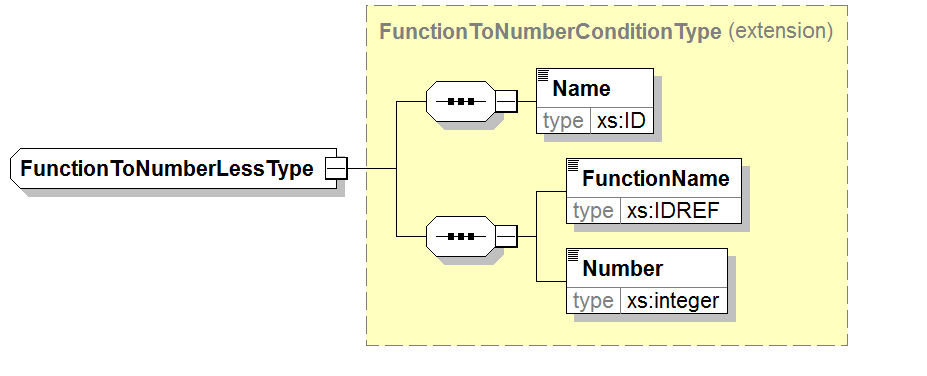
\includegraphics[width=1\linewidth]{images/XMLSPYDiagrams/FunctionToNumberLessType.png}
%        \caption{\textsf{FunctionToNumberLessType} for comparing PDDL functions with numbers using the mathematical symbol ``$<$".}
%        \label{fig:FunctionToNumberLessType}
%        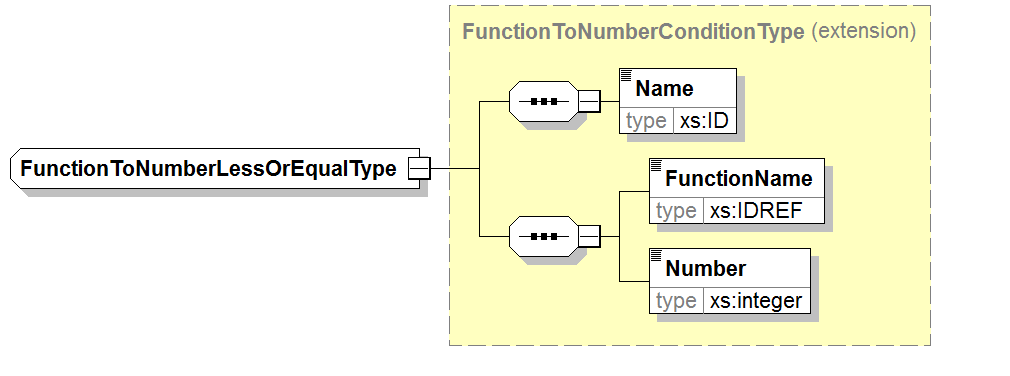
\includegraphics[width=1\linewidth]{images/XMLSPYDiagrams/FunctionToNumberLessOrEqualType.png}
%        \caption{\textsf{FunctionToNumberLessOrEqualType} for comparing PDDL functions with numbers using the mathematical symbol ``$\leq$".}
%        \label{fig:FunctionToNumberLessOrEqualType}
%        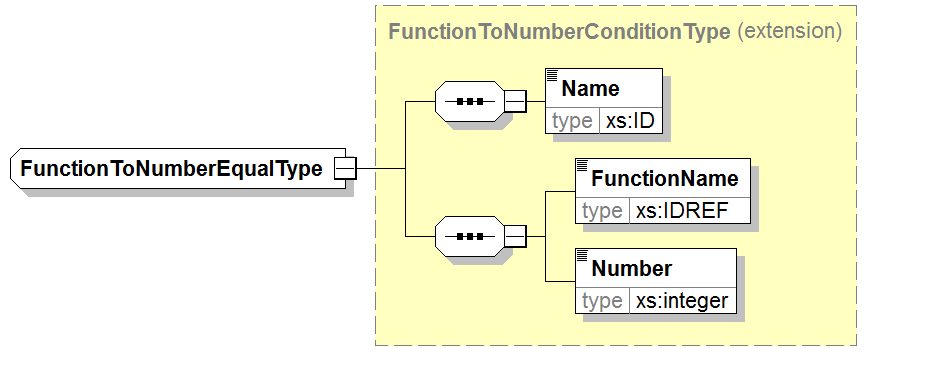
\includegraphics[width=1\linewidth]{images/XMLSPYDiagrams/FunctionToNumberEqualType.png}
%        \caption{\textsf{FunctionToNumberEqualType} for comparing PDDL functions with numbers using the mathematical symbol ``$=$".}
%        \label{fig:FunctionToNumberEqualType}
%        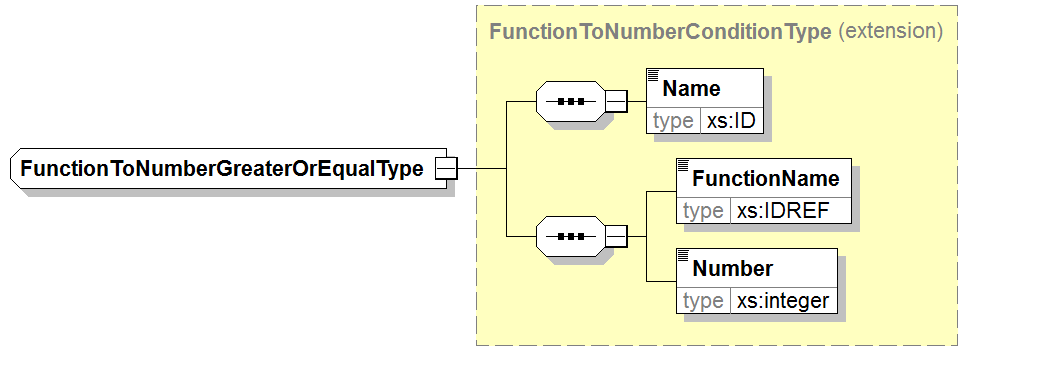
\includegraphics[width=1\linewidth]{images/XMLSPYDiagrams/FunctionToNumberGreaterOrEqualType.png}
%        \caption{\textsf{FunctionToNumberGreaterOrEqualType} for comparing PDDL functions with numbers using the mathematical symbol ``$\geq$".}
%        \label{fig:FunctionToNumberGreaterOrEqualType}
%        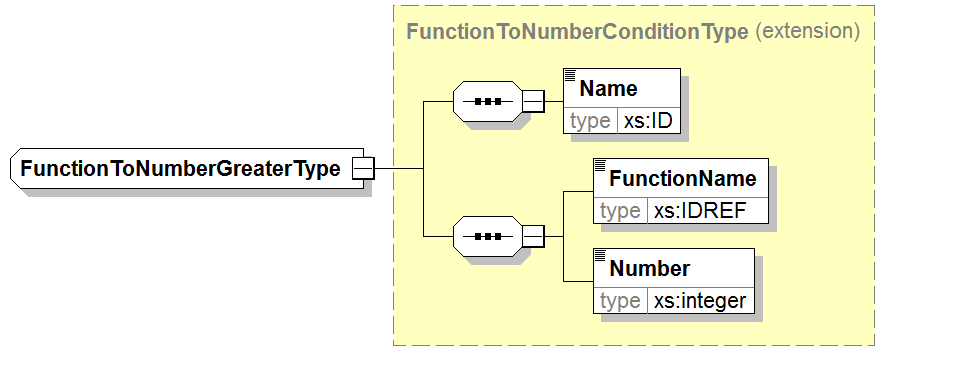
\includegraphics[width=1\linewidth]{images/XMLSPYDiagrams/FunctionToNumberGreaterType.png}
%        \caption{\textsf{FunctionToNumberGreaterType} for comparing PDDL functions with numbers using the mathematical symbol ``$>$".}
%        \label{fig:FunctionToNumberGreaterType}
%        \end{subfigure}
%        \caption{Subtypes of \textsf{FunctionToNumberConditionType}.}
%        \label{fig:fig}
%        \end{figure}

\end{itemize}
\item \emph{Effect}: The effect section of a PDDL action is modeled with \textsf{EffectType} (see Figure~\ref{fig:EffectType}). \textsf{EffectType} extends \textsf{DataThingType}. \textsf{EffectType} consists of a unique name (inherited), optional references to positive predicates, optional definitions of negative predicates, and optional references to function operations (identified with \emph{Increase} and \emph{Decrease}). Information on each component of \textsf{EffectType} is given below.
    \begin{figure}[t!b!]
    \centering
    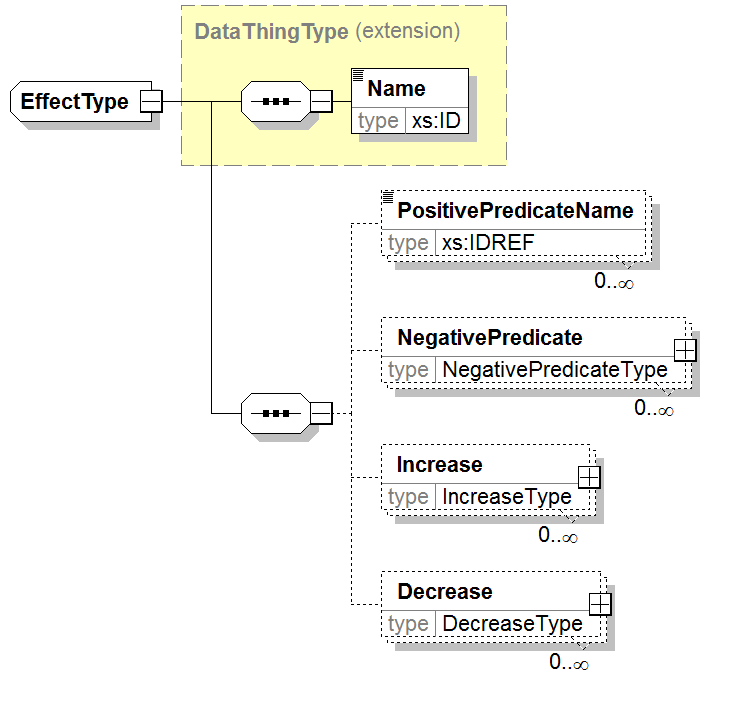
\includegraphics[width=.5\linewidth]{images/XMLSPYDiagrams/EffectType.png}
    \caption{\textsf{EffectType} for modeling PDDL actions' effects.}
    \label{fig:EffectType}
    \end{figure}

    \begin{itemize}
    \item \emph{PositivePredicateName} is a reference to a positive predicate. This requires that the referenced \textsf{PositivePredicateType} is already defined.
    \item \emph{NegativePredicate} describes a \textsf{NegativePredicateType} (see Figure~\ref{fig:NegativePredicateType}). A \textsf{NegativePredicateType} extends \textsf{DataThingType}  and models the negation of a predicate. A \textsf{NegativePredicateType} consists of a name (inherited) and a reference to a positive predicate.
        \begin{figure}[htb!]
        \centering
        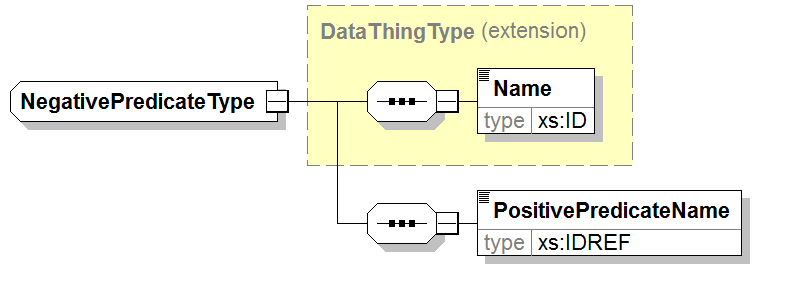
\includegraphics[width=.5\linewidth]{images/XMLSPYDiagrams/NegativePredicateType.png}
        \caption{\textsf{NegativePredicateType} for modeling the negation of PDDL positive predicates.}
        \label{fig:NegativePredicateType}
        \end{figure}
    \item Function operations are arithmetic expressions on a \textsf{FunctionType}. Effects can make use of a selection of assignment operations in order to update the values of primitive numeric expressions. The value of a function can be decreased or increased by a certain amount. Function operations are modeled with \textsf{FunctionOperationType} which extends \textsf{DataThingType}. Subtypes of \textsf{FunctionOperationType} are \textsf{IncreaseType} (see Figure~\ref{fig:IncreaseType}) and \textsf{DecreaseType} (see Figure~\ref{fig:DecreaseType}). \textsf{IncreaseType} and \textsf{DecreaseType} consist of a unique name (inherited), a reference to a function (identified with \emph{FunctionName}), and a value (identified by \emph{Value}) by which the function is increased or decreased, respectively. An instance of \textsf{DecreaseType} can be found at line 43 in Figure~\ref{fig:domain} where the function is \texttt{(quantity-of-kittrays-in-lbwekt ?lbwekt)} and the value is \texttt{1}.



\begin{figure}[htb!]
\begin{subfigure}{.5\textwidth}
  \centering
  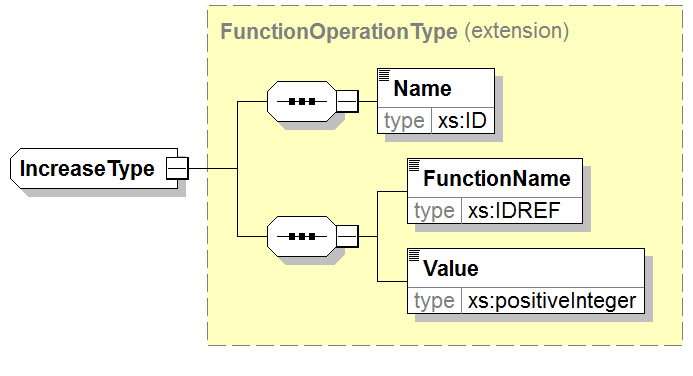
\includegraphics[width=.7\linewidth]{images/XMLSPYDiagrams/IncreaseType.png}
  \caption{\textsf{IncreaseType}.}
  \label{fig:IncreaseType}
\end{subfigure}%
\begin{subfigure}{.5\textwidth}
  \centering
  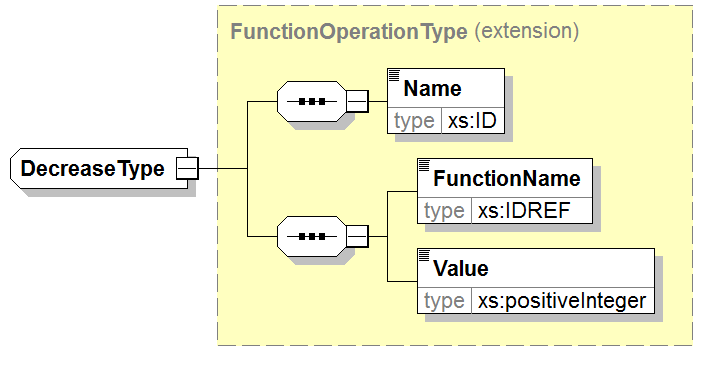
\includegraphics[width=.7\linewidth]{images/XMLSPYDiagrams/DecreaseType.png}
  \caption{\textsf{DecreaseType}.}
  \label{fig:DecreaseType}
\end{subfigure}

\caption{Subtypes of \textsf{FunctionOperationType}.}
\label{fig:fig}
\end{figure}
    \end{itemize}
\end{itemize}
\end{itemize}
%\begin{figure}[htb!]
%\begin{subfigure}{.4\textwidth}
%  \begin{minipage}[t]{0.4\textwidth}
%\begin{mylisting}
%\begin{Verbatim}[commandchars=\\\{\},fontsize=\scriptsize, numbers=left, numbersep=0.5pt]
%<?xml version="1.0" encoding="UTF-8"?>
%<SOAP
% xmlns:xsi="http://www.w3.org/2001/
% XMLSchema-instance"
% xsi:noNamespaceSchemaLocation="../
% xmlSchemas/soap.xsd">
% <Name>soap</Name>
% <Domain>
%  <Name>kitting-domain</Name>
%  <Requirement>action-costs</Requirement>
%  ...
%  <Variable>EndEffector</Variable>
%  ...
%  <PositivePredicate>
%   <Name>endEffector-is-for-kitTraySKU</Name>
%   <ReferenceParameter>
%    EndEffector
%   </ReferenceParameter>
%   <TargetParameter>
%    StockKeepingUnit
%   </TargetParameter>
%  </PositivePredicate>
%  ...
%  <Function>
%   <Name>
%    quantity-of-kittrays-in-lbwekt
%   </Name>
%   <ReferenceParameter>
%    LargeBoxWithEmptyKitTrays
%   </ReferenceParameter>
%  </Function>
%    ...
%  <Action>
%   <Name>take-kitTray</Name>
%   <ActionParameterSet>
%    <Name>take-kitTray-parameter-1</Name>
%    <ActionParameter>Robot</ActionParameter>
%    <ActionParameterPosition>
%     1
%    </ActionParameterPosition>
%   </ActionParameterSet>
%   <ActionParameterSet>
%    <Name>take-kitTray-parameter-2</Name>
%    <ActionParameter>KitTray</ActionParameter>
%    <ActionParameterPosition>
%     2
%    </ActionParameterPosition>
%   </ActionParameterSet>
%   <ActionParameterSet>
%    <Name>take-kitTray-parameter-3</Name>
%    <ActionParameter>
%     LargeBoxWithEmptyKitTrays
%    </ActionParameter>
%    <ActionParameterPosition>
%     3
%    </ActionParameterPosition>
%   </ActionParameterSet>
%   <ActionParameterSet>
%   <Name>take-kitTray-parameter-4</Name>
%   <ActionParameter>
%    EndEffector
%   </ActionParameter>
%   <ActionParameterPosition>
%    4
%   </ActionParameterPosition>
%  </ActionParameterSet>
%\end{Verbatim}
%\end{mylisting}
%\end{minipage}
%\end{subfigure}%
%\begin{subfigure}{.5\textwidth}
% \begin{minipage}[t]{0.5\textwidth}
%\begin{mylisting}
%\begin{Verbatim}[commandchars=\\\{\},fontsize=\scriptsize, numbers=left, firstnumber=last,numbersep=2pt]
%   <ActionParameterSet>
%    <Name>take-kitTray-parameter-StockKeepingUnit</Name>
%    <ActionParameter>StockKeepingUnit</ActionParameter>
%    <ActionParameterPosition>5</ActionParameterPosition>
%   </ActionParameterSet>
%
%   <Precondition>
%    <Name>take-kitTray-precondition</Name>
%    <PositivePredicateName>
%     endEffector-is-for-kitTraySKU
%    </PositivePredicateName>
%    <PositivePredicateName>
%     robot-has-endEffector
%    </PositivePredicateName>
%    <PositivePredicateName>
%     endEffector-has-no-heldObject
%    </PositivePredicateName>
%    <PositivePredicateName>
%     kitTray-has-physicalLocation-refObject-lbwekt
%    </PositivePredicateName>
%    <PositivePredicateName>
%     kitTray-has-skuObject-sku
%    </PositivePredicateName>
%    <PositivePredicateName>
%     endEffector-has-physicalLocation-refObject-robot
%    </PositivePredicateName>
%    <FunctionToNumberGreater>
%     <Name>take-kitTray-FunctionToNumberGreater</Name>
%     <FunctionName>quantity-of-kittrays-in-lbwekt</FunctionName>
%     <Number>0</Number>
%    </FunctionToNumberGreater>
%   </Precondition>
%   <Effect>
%    <Name>take-kitTray-effect</Name>
%    <PositivePredicateName>
%     kitTray-has-physicalLocation-refObject-endEffector
%    </PositivePredicateName>
%    <PositivePredicateName>
%     endEffector-has-heldObject-kitTray
%    </PositivePredicateName>
%    <NegativePredicate>
%     <Name>not-kitTray-has-physicalLocation-refObject-lbwekt</Name>
%     <PositivePredicateName>
%      kitTray-has-physicalLocation-refObject-lbwekt
%     </PositivePredicateName>
%    </NegativePredicate>
%    <NegativePredicate>
%     <Name>not-endEffector-has-no-heldObject</Name>
%     <PositivePredicateName>
%      endEffector-has-no-heldObject
%     </PositivePredicateName>
%    </NegativePredicate>
%    <Decrease>
%     <Name>take-kitTray-decrease</Name>
%     <FunctionName>quantity-of-kittrays-in-lbwekt</FunctionName>
%     <Value>1</Value>
%    </Decrease>
%   </Effect>
%  </Action>
%  ...
% </Domain>
%</SOAP>
%         \end{Verbatim}
%\end{mylisting}
%\end{minipage}
%\end{subfigure}
%\caption{XML instance file. Ellipses represent information that have been omitted on purpose to simplify the illustration of the XML instance file.}
%\label{fig:xml}
%\end{figure}





\section{Automatic Generation of PDDL Files}
\label{section:java-tool}
Once the schema models for PDDL were in place, an XML instance file that conforms to the schema models was developed. %An excerpt of the XML instance file that conforms to \textsf{SOAP} XML schema file is depicted in Figure~\ref{fig:xml}. 
Under the XML standards, an XML data file conforming to an XML schema must be in a different format than the schema and must contain different sorts of statements. An XML statement naming the XML schema file to which an instance file corresponds is normally given near the beginning of the instance file. Many different instance files may correspond to the same schema. The form of an XML instance file is a tree in which instances of the elements of each type are textually inside the instance of the type. Schema models and the XML instance file are used by a set of tools to automatically generate a set of OWL files. The tools required to perform this mechanism were developed by one of the authors at NIST. More information about this set of tools can be found in~\cite{Balakirsky.NISTIR.2013}.



To date, the PDDL domain and problem files are hand generated. An expert needs to write these two files and it takes a considerable amount of time to complete these files.
A Java-based tool was developed in this effort to automatically and dynamically build these PDDL files. The tool was developed in Java because of its inherent ability to interface with OWL API~\cite{OWLAPI}. The OWL API is a Java API and reference implementation for creating, manipulating
and serialising OWL Ontologies. Please note that the use of the language and the API is the authors' choice and the same result may be obtained differently.



\subsection{Automatic Generation of the Domain File}

The generation of the PDDL domain file is performed by reading the OWL classes from the \textsf{SOAP} OWL file. Since a PDDL domain file stays unchanged during a replanning process, the blueprint of the PDDL domain file is programmed. The tool only needs to access each part of this blueprint from the ontology and outputs this information in a PDDL domain file. Figure~\ref{fig:domaingeneration} shows the components that are read from the SOAP OWL file, stored in the program, and written in the PDDL domain file.
\begin{figure}[htb!]
\centering
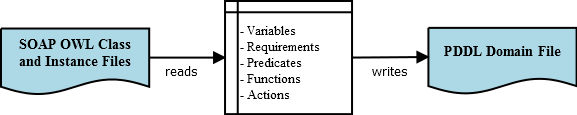
\includegraphics[width=.7\linewidth]{images/domain.png}
\caption{Generation of a PDDL domain file.}
\label{fig:domaingeneration}
\end{figure}

\subsection{Automatic Generation of the Problem File}
The PDDL problem file consists of dynamically generated \texttt{init} and \texttt{goal} states. The predicates and function initializations that go in the \texttt{goal} state are built from the OWL goal instance file. This information is then written in the \texttt{goal} state of the problem file. The \texttt{goal} state for a given kit to build is unchanged during replanning and plan repair. The \texttt{init} state allows successful replanning and plan repair processes where the current state of the world becomes the new \texttt{init} state of the problem file. The tool has the ability to read the \textsf{SOAP} OWL class and instance files along with the OWL \texttt{init} instance files to write only predicates that are true in the \texttt{init} state. Functions are also initialized in the \texttt{init} state. A mapping for each predicate and for the initialization of each function is programmed.



\subsubsection{Building and Writing Predicates}
\IncMargin{0.5em}
\begin{algorithm}
\BlankLine
\emph{read OWLClass:PartsTray in OWL init instance file}\;
\emph{build $\mathrm{partsTrayNodeSet=[partsTray_i]_{i=1}^{i=n}}$}\;
\If(){$\mathrm{partsTrayNodeSet}$ is not empty}{\For{each $\mathrm{partsTray_i}$}{build $\mathrm{partNodeSet=[part_j:(kit_i,hasPartsVessel\_Part)]_{i=1,j=1}^{i=n,j=o}}$\;
\If(){$\mathrm{partNodeSet}$ is not empty}{
\For{each $\mathrm{part_j}$}{write (partsVessel-has-part $\mathrm{partsTray_i}$ $\mathrm{part_j}$)$\mathrm{_{i=1, j=1}^{i=n, j=o}}$}}}}
\caption{Building a predicate}\label{algo}
\end{algorithm}\DecMargin{0.5em}
As mentioned earlier, a mapping is set for each predicate that is contained in the \texttt{predicates} section of a domain file. The mapping reads OWL files to fetch the information that is relevant for a given predicate. For instance, the predicate \texttt{partsVessel-has-part part\_a\_tray part\_a\_1} (line 26 in Figure~\ref{fig:problem}) is true if the parts tray \texttt{part\_a\_tray} contains the part \texttt{part\_a\_1}. The algorithm developed to build and write this predicate in the \textsf{init} section of the problem file is described in Algorithm~\ref{algo}. The algorithm reads the class \emph{PartsTray} from the OWL \textsf{init} instance file, retrieves all the individuals of this class (line 1), and inserts the individuals in a list of parts trays $\mathrm{partsTrayNodeSet}$ (line 2). For each $\mathrm{partsTray_i}$ in $\mathrm{partsTrayNodeSet}$, the algorithm uses the object property $\mathrm{hasPartsVessel\_Part}$ to retrieve all the parts (line 4). The domain of the object property $\mathrm{hasPartsVessel\_Part}$ is the OWL class \emph{PartsTray} and its range is the OWL class \emph{Part}, that is, given a parts tray, $\mathrm{hasPartsVessel\_Part}$ fetches all the parts contained in this parts tray. Each $\mathrm{part_i}$ is then stored in a list of parts $\mathrm{partNodeSet}$ (line 5). Finally, the algorithm writes the predicate \texttt{partsVessel-has-part} with proper OWL individuals as parameters, i.e., \texttt{part\_a\_tray} and \texttt{part\_a\_1} in this example.

Note that if the condition at line 3 is not satisfied, i.e., if there are no parts trays in the ontology, this predicate is not written in the \textsf{init} state of the problem file. Similarly, if $\mathrm{partNodeSet}$ is empty, i.e., there is no parts in the parts tray, the predicate is also not written.



\subsubsection{Initializing Functions}
All the functions defined in the domain file are initialized in the \textsf{init} section of the problem file. If a function has a reference parameter, the function is initialized for each instance of the reference parameter. For instance, the function \texttt{(quantity-of-parts-in-partstray ?partstray - PartsTray)} sets the number of parts in a parts tray. This function is initialized for each parts tray found in the OWL init instance file, i.e., for \texttt{part\_a\_tray} and \texttt{part\_b\_tray} as shown in Figure~\ref{fig:problem} at line 29 and at line 30, respectively.

The value that is used to initialize a function is either retrieved from the OWL init instance file or computed using data from the OWL init instance file. For instance, initializing the function \texttt{(capacity-of-kits-in-lbwk ?lbwk - LargeBoxWithKits)} (line 25 in Figure~\ref{fig:domain}) requires a value which is retrieved, while the value that is used to initialize the function \texttt{(quantity-of-parts-in-partstray ?partstray - PartsTray)} (line 18 in Figure~\ref{fig:domain}) is computed. The algorithm that builds and writes the former function is illustrated in Algorithm~\ref{algo:function1} and the algorithm that builds and writes the latter function is illustrated in Algorithm~\ref{algo:function2}. Explanations for Algorithm~\ref{algo:function1} and Algorithm~\ref{algo:function2} are given as follows:
\begin{itemize}
\item Algorithm~\ref{algo:function1}: First, the algorithm reads the OWL \texttt{init} instance file (line 1), retrieves all OWL individuals of type \emph{LargeBoxWithKits}, and stores them in the list $\mathrm{largeBoxWithKitsNodeSet}$ (line 2). If the list $\mathrm{largeBoxWithKitsNodeSet}$ is not empty (line 3), for each $\mathrm{largeBoxWithKits_i}$, the number of kits that the large box with kits $\mathrm{largeBoxWithKits_i}$ can contain ($\mathrm{lbwkCapacity}$) is retrieved with the OWL data property $\mathrm{hasLargeWithKits\_Capacity}$ (line 5). Finally, the function is written with $\mathrm{largeBoxWithKits_i}$ as the reference parameter and $\mathrm{lbwkCapacity}$ as the initial value (line 6).

    \IncMargin{0.5em}
\begin{algorithm}
\BlankLine
\emph{read OWLClass:LargeBoxWithKits in OWL init instance file}\;
\emph{build $\mathrm{largeBoxWithKitsNodeSet=[largeBoxWithKits_i]_{i=1}^{i=n}}$}\;
\If(){$\mathrm{largeBoxWithKitsNodeSet}$ is not empty}{\For{each $\mathrm{largeBoxWithKits_i}$}{
\emph{$\mathrm{int}$ $\mathrm{lbwkCapacity=[largeBoxWithKits_i,hasLargeWithKits\_Capacity]_{i=1}^{i=n}}$}\;
write (= (capacity-of-kits-in-lbwk $\mathrm{largeBoxWithKits_i}$) $\mathrm{lbwkCapacity}$)$\mathrm{_{i=1}^{i=n}}$}}
\caption{Retrieved value for function initialization.}\label{algo:function1}
\end{algorithm}\DecMargin{0.5em}
\item Algorithm~\ref{algo:function2}: First, the algorithm reads the OWL \texttt{init} instance file (line 1), retrieves all OWL individuals of type \emph{PartsTray}, and stores them in the list $\mathrm{partsTrayNodeSet}$ (line 2). For each parts tray $\mathrm{partsTray_i}$, the number of parts $\mathrm{NumberOfParts}$ in $\mathrm{partsTray_i}$ is set to 0 (line 5). The algorithm then retrieves all the parts for  each $\mathrm{partsTray_i}$ and stores them in the list $\mathrm{partNodeSet}$ (line 6). $\mathrm{NumberOfParts}$ is incremented each time a part is found in $\mathrm{partNodeSet}$ (line 9). Finally, for each $\mathrm{partsTray_i}$, the function is initialized, where $\mathrm{partsTray_i}$ is the reference parameter and $\mathrm{NumberOfParts}$ is the number of parts in $\mathrm{partsTray_i}$ (line 12).
    \IncMargin{0.5em}
\begin{algorithm}
\BlankLine
\emph{read OWLClass:PartsTray in OWL init instance file}\;
\emph{build $\mathrm{partsTrayNodeSet=[partsTray_i]_{i=1}^{i=n}}$}\;
\If(){$\mathrm{partsTrayNodeSet}$ is not empty}{\For{each $\mathrm{partsTray_i}$}{set $\mathrm{numberOfParts=0}$\;
\emph{build $\mathrm{partNodeSet=[part_j:(partsTray_i,hasPartsVessel\_Part)]_{i=1,j=1}^{i=n,j=o}}$}\;
\If(){$\mathrm{partNodeSet}$ is not empty}{\For{each $\mathrm{part_j}$}{$\mathrm{numberOfParts++}$}}write (= (quantity-of-parts-in-partstray $\mathrm{partsTray_i}$) $\mathrm{numberOfParts}$)$\mathrm{_{i=1}^{i=n}}$}}
\caption{Computed value for function initialization.}\label{algo:function2}
\end{algorithm}\DecMargin{0.5em}
\end{itemize}





\section{Conclusion and Future Work}
\label{section:conclusion}

This paper presented the latest tasks in the area of kit building, part of the ``Agility Performance of Robotic Systems" (APRS) project at the National Institute of Standards and Technology (NIST). The authors presented models in the XML Schema Definition Language (XSDL) for PDDL structures. These models are used to generate a set of OWL files. The generated OWL files are employed to automatically and dynamically generate PDDL domain and problem files. This function allows replanning and plan repair when action failures are encountered during the kitting process. The automatic and dynamic generation of PDDL files is an attempt at bringing agility and flexibility in the APRS project. As mentioned in Section~\ref{section:architecture}, a MySQL database is updated with information on the current state of the world as a kitting process is performed. The next step in this effort is to generate the PDDL problem file with data directly retrieved from the MySQL database while the PDDL domain file will still be generated from a set of OWL files.
\section{Disclaimer}
No approval or endorsement of any commercial product by the authors is intended or implied. Certain commercial software systems are identified in this paper to facilitate understanding. Such identification does not imply that these software systems are necessarily the best available for the purpose.

%% References with BibTeX database:

\bibliographystyle{elsarticle-num}
\bibliography{RCIM-KOOTBALLY}

%% Authors are advised to use a BibTeX database file for their reference list.
%% The provided style file elsarticle-num.bst formats references in the required Procedia style

%% For references without a BibTeX database:

% \begin{thebibliography}{00}

%% \bibitem must have the following form:
%%   \bibitem{key}...
%%

% \bibitem{}

% \end{thebibliography}

\end{document}

%%
%% End of file `ecrc-template.tex'. 